% Soubory musí být v kódování, které je nastaveno v příkazu \usepackage[...]{inputenc}

\documentclass[%        Základní nastavení
  %draft,    				  % Testovací překlad
  12pt,       				% Velikost základního písma je 12 bodů
	t,                  % obsah slajdů bude vždy začínat od shora (nebude vertikálně centrovaný)
	aspectratio=1610,   % poměr stran bude 16:10 (všechny projektory v učebnách na Technické 12 Brno),
	                    % další volby jsou 43, 149, 169, 54, 32.
	unicode,						% Záložky a informace budou v kódování unicode
]{beamer}				    	% Dokument třídy 'zpráva', vhodná pro sazbu závěrečných prací s kapitolami
%\usepackage{etex}

\usepackage[utf8]		  % Kódování zdrojových souborů je v UTF-8
	{inputenc}					% Balíček pro nastavení kódování zdrojových souborů
	
\usepackage{graphicx} % Balíček 'graphicx' pro vkládání obrázků
											% Nutné pro vložení logotypů školy a fakulty

\usepackage[          % Balíček 'acronym' pro sazby zkratek a symbolů
	nohyperlinks				% Nebudou tvořeny hypertextové odkazy do seznamu zkratek
]{acronym}						
											% Nutné pro použití prostředí 'acronym' balíčku 'thesis'

%% Balíček hyperref je volán třídou beamer automaticky, proto není třeba následujícího kódu:
%\usepackage[
%	breaklinks=true,		% Hypertextové odkazy mohou obsahovat zalomení řádku
%	hypertexnames=false % Názvy hypertextových odkazů budou tvořeny
%											% nezávisle na názvech TeXu
%]{hyperref}						% Balíček 'hyperref' pro sazbu hypertextových odkazů
%											% Nutné pro použití příkazu 'nastavenipdf' balíčku 'thesis'

\usepackage{cmap} 		% Balíček cmap zajišťuje, že PDF vytvořené `pdflatexem' je
											% plně "prohledávatelné" a "kopírovatelné"

%\usepackage{upgreek}	% Balíček pro sazbu stojatých řeckých písmem
											%% např. stojaté pí: \uppi
											%% např. stojaté mí: \upmu (použitelné třeba v mikrometrech)
											%% pozor, grafická nekompatibilita s fonty typu Computer Modern!

%\usepackage{amsmath} %balíček pro sabu náročnější matematiky

\usepackage{booktabs} % Balíček, který umožňuje v tabulce používat
                      % příkazy \toprule, \midrule, \bottomrule


%%%%%%%%%%%%%%%%%%%%%%%%%%%%%%%%%%%%%%%%%%%%%%%%%%%%%%%%%%%%%%%%%
%%%%%%      Definice informací o dokumentu             %%%%%%%%%%
%%%%%%%%%%%%%%%%%%%%%%%%%%%%%%%%%%%%%%%%%%%%%%%%%%%%%%%%%%%%%%%%%

% V tomto souboru se nastavují téměř veškeré informace, proměnné mezi studenty:
% jméno, název práce, pohlaví atd.
% Tento soubor je SDÍLENÝ mezi textem práce a prezentací k obhajobě -- netřeba něco nastavovat na dvou místech.

\usepackage[
%%% Z následujících voleb jazyka lze použít pouze jednu
  czech-english,		% originální jazyk je čeština, překlad je anglicky (výchozí)
  %english-czech,	% originální jazyk je angličtina, překlad je česky
  %slovak-english,	% originální jazyk je slovenština, překlad je anglicky
  %english-slovak,	% originální jazyk je angličtina, překlad je slovensky
%
%%% Z následujících voleb typu práce lze použít pouze jednu
  %semestral,		  % semestrální práce (nesází se abstrakty, prohlášení, poděkování) (výchozí)
  %bachelor,			%	bakalářská práce
  master,			  % diplomová práce
  %treatise,			% pojednání o disertační práci
  %doctoral,			% disertační práce
%
%%% Z následujících voleb zarovnání objektů lze použít pouze jednu
%  left,				  % rovnice a popisky plovoucích objektů budou zarovnány vlevo
	center,			    % rovnice a popisky plovoucích objektů budou zarovnány na střed (vychozi)
%
]{thesis}   % Balíček pro sazbu studentských prací


%%% Jméno a příjmení autora ve tvaru
%  [tituly před jménem]{Křestní}{Příjmení}[tituly za jménem]
% Pokud osoba nemá titul před/za jménem, smažte celý řetězec '[...]'
\author[Bc.]{Filip}{Paul}

%%% Identifikační číslo autora (VUT ID)
\butid{211 538}

%%% Pohlaví autora/autorky
% (nepoužije se ve variantě english-czech ani english-slovak)
% Číselná hodnota: 1...žena, 0...muž
\gender{0}

%%% Jméno a příjmení vedoucího/školitele včetně titulů
%  [tituly před jménem]{Křestní}{Příjmení}[tituly za jménem]
% Pokud osoba nemá titul před/za jménem, smažte celý řetězec '[...]'
\advisor[prof.\ Dr.\ Ing.]{Zdeněk}{Kolka}

%%% Jméno a příjmení oponenta včetně titulů
%  [tituly před jménem]{Křestní}{Příjmení}[tituly za jménem]
% Pokud osoba nemá titul před/za jménem, smažte celý řetězec '[...]'
% Nastavení oponenta se uplatní pouze v prezentaci k obhajobě;
% v případě, že nechcete, aby se na titulním snímku prezentace zobrazoval oponent, pouze příkaz zakomentujte;
% u obhajoby semestrální práce se oponent nezobrazuje (jelikož neexistuje)
% U dizertační práce jsou typicky dva až tři oponenti. Pokud je chcete mít na titulním slajdu, prosím ručně odkomentujte a upravte jejich jména v definici "VUT title page" v souboru thesis.sty.
\opponent[doc.\ Mgr.]{Křestní}{Příjmení}[Ph.D.]

%%% Název práce
%  Parametr ve složených závorkách {} je název v originálním jazyce,
%  parametr v hranatých závorkách [] je překlad (podle toho jaký je originální jazyk).
%  V případě, že název Vaší práce je dlouhý a nevleze se celý do zápatí prezentace, použijte příkaz
%  \def\insertshorttitle{Zkác.\ náz.\ práce}
%  kde jako parametr vyplníte zkrácený název. Pokud nechcete zkracovat název, budete muset předefinovat,
%  jak se vytváří patička slidu. Viz odkaz: https://bit.ly/3EJTp5A
\title[Title of Student's Thesis]{Výrobní tester}

%%% Označení oboru studia
%  Parametr ve složených závorkách {} je název oboru v originálním jazyce,
%  parametr v hranatých závorkách [] je překlad
\specialization[Teleinformatics]{Teleinformatika}

%%% Označení ústavu
%  Parametr ve složených závorkách {} je název ústavu v originálním jazyce,
%  parametr v hranatých závorkách [] je překlad
%\department[Department of Control and Instrumentation]{Ústav automatizace a měřicí techniky}
%\department[Department of Biomedical Engineering]{Ústav biomedicínského inženýrství}
%\department[Department of Electrical Power Engineering]{Ústav elektroenergetiky}
%\department[Department of Electrical and Electronic Technology]{Ústav elektrotechnologie}
%\department[Department of Physics]{Ústav fyziky}
%\department[Department of Foreign Languages]{Ústav jazyků}
%\department[Department of Mathematics]{Ústav matematiky}
%\department[Department of Microelectronics]{Ústav mikroelektroniky}
\department[Department of Radio Electronics]{Ústav radioelektroniky}
%\department[Department of Theoretical and Experimental Electrical Engineering]{Ústav teoretické a experimentální elektrotechniky}
%\department[Department of Telecommunications]{Ústav telekomunikací}
%\department[Department of Power Electrical and Electronic Engineering]{Ústav výkonové elektrotechniky a elektroniky}

%%% Označení fakulty
%  Parametr ve složených závorkách {} je název fakulty v originálním jazyce,
%  parametr v hranatých závorkách [] je překlad
%\faculty[Faculty of Architecture]{Fakulta architektury}
\faculty[Faculty of Electrical Engineering and~Communication]{Fakulta elektrotechniky a~komunikačních technologií}
%\faculty[Faculty of Chemistry]{Fakulta chemická}
%\faculty[Faculty of Information Technology]{Fakulta informačních technologií}
%\faculty[Faculty of Business and Management]{Fakulta podnikatelská}
%\faculty[Faculty of Civil Engineering]{Fakulta stavební}
%\faculty[Faculty of Mechanical Engineering]{Fakulta strojního inženýrství}
%\faculty[Faculty of Fine Arts]{Fakulta výtvarných umění}
%
%Nastavení logotypu (v hranatych zavorkach zkracene logo, ve slozenych plne):
\facultylogo[logo/FEKT_zkratka_barevne_PANTONE_CZ]{logo/FEKT_zkratka_barevne_PANTONE_CZ}

%%% Rok odevzdání práce
\graduateyear{2023}
%%% Akademický rok odevzdání práce
\academicyear{2022/23}

%%% Datum obhajoby (uplatní se pouze v prezentaci k obhajobě)
\date{6.\,6.\,2023} 

%%% Místo obhajoby
% Na titulních stránkách bude automaticky vysázeno VELKÝMI písmeny (pokud tyto stránky sází šablona)
\city{Brno}

%%% Abstrakt
\abstract[%
The diploma thesis deals with the design and implementation of a device,
which is used to verify the internal electrical wiring of ICT testers.
Wiring is verified by measuring the resistance between individual test points.
ICT testers can contain thousands of connections. The device should be able to identify wiring errors,
inform the operator about the error and propose a relevant solution.

]{%
Diplomová práce se zabývá návrhem a realizací zařízení, které slouží k ověření 
správnosti vnitřního elektrického zapojení ICT testerů. Správnost zapojení
je ověřována měřením odporu mezi jednotlivýmy testovacími body.
ICT testery mohou obsahovat řádově tisíce propojení. Navrhované zařízení by mělo být
schopno identifikovat chyby propojení a následně navrhnout vhodné řešení.

}

%%% Klíčová slova
\keywrds[%
In-Circuit Testing (ICT), Fixture, Testpoint, Test probes, End Of Line (EOL).
]{%
In-Circuit Testing (ICT), Fixture, Testovací body, Testovací jehly, End Of Line (EOL).
}

%%% Poděkování
\acknowledgement{%
Rád bych poděkoval vedoucímu diplomové práce
panu Prof. Dr. Ing. Zdeňku Kolkovi za odborné vedení,
konzultace, trpělivost a~podnětné návrhy k~práci.
}%      % v tomto souboru doplňte údaje o sobě, o názvu práce...
                       % (tento soubor je sdílený s textem práce)

%%%%%%%%%%%%%%%%%%%%%%%%%%%%%%%%%%%%%%%%%%%%%%%%%%%%%%%%%%%%%%%%%%%%%%%%

%%%%%%%%%%%%%%%%%%%%%%%%%%%%%%%%%%%%%%%%%%%%%%%%%%%%%%%%%%%%%%%%%%%%%%%%
%%%%%%     Nastavení polí ve Vlastnostech dokumentu PDF      %%%%%%%%%%%
%%%%%%%%%%%%%%%%%%%%%%%%%%%%%%%%%%%%%%%%%%%%%%%%%%%%%%%%%%%%%%%%%%%%%%%%
%% Při vloženém balíčku 'hyperref' lze použít příkaz '\pdfsettings'
\pdfsettings
%  Nastavení polí je možné provést také ručně příkazem:
%\hypersetup{
%  pdftitle={Název studentské práce},    	% Pole 'Document Title'
%  pdfauthor={Autor studenstké práce},   	% Pole 'Author'
%  pdfsubject={Typ práce}, 						  	% Pole 'Subject'
%  pdfkeywords={Klíčová slova}           	% Pole 'Keywords'
%}
\hypersetup{pdfpagemode=FullScreen}       % otevření rovnou v režimu celé obrazovky
%%%%%%%%%%%%%%%%%%%%%%%%%%%%%%%%%%%%%%%%%%%%%%%%%%%%%%%%%%%%%%%%%%%%%%%

\usetheme{VUT} 				% barvy a rozložení prezentace odpovídající VUT FEKT
% alternativně lze použít jiná berevná témata, ale bez záruky. Například: 
%\usetheme{Darmstadt} \usecolortheme{default2}
\logoheader					% vytvoření zkráceného loga VUT FEKT v hlavičce slajdu, nechte odkomentované



\begin{document}

% v případě zakomentování následujícího se zobrazí v pravém dolním rohu slajdů klikatelné navigační symboly 
\disablenavigationsymbols

% titulní snímek, vysazen bez horních, dolních a postranních lišt (volba plain),
% není tak vysazen ani nadpis snímku
\maketitle

%%%%%%%%%%%%%%%%%%%%%%%%%%%%%%%%%%%%%%%%%%%%%%%%%%%%%%%%%%%%%%%%%%%%%%%

\begin{frame} 
	% nadpis snímku
	\frametitle{Cíle práce}
	\begin{figure}[ht!]
		\centering
		\begin{minipage}{0.3\textwidth}
			\vspace*{-3cm}
			\begin{itemize}
				\item ICT tester
				\item Fixture
				\item Měření odporu
				\item Škálovatelnost
				\item Rychlost
			\end{itemize}
		\end{minipage}
		\begin{minipage}{0.65\textwidth}
		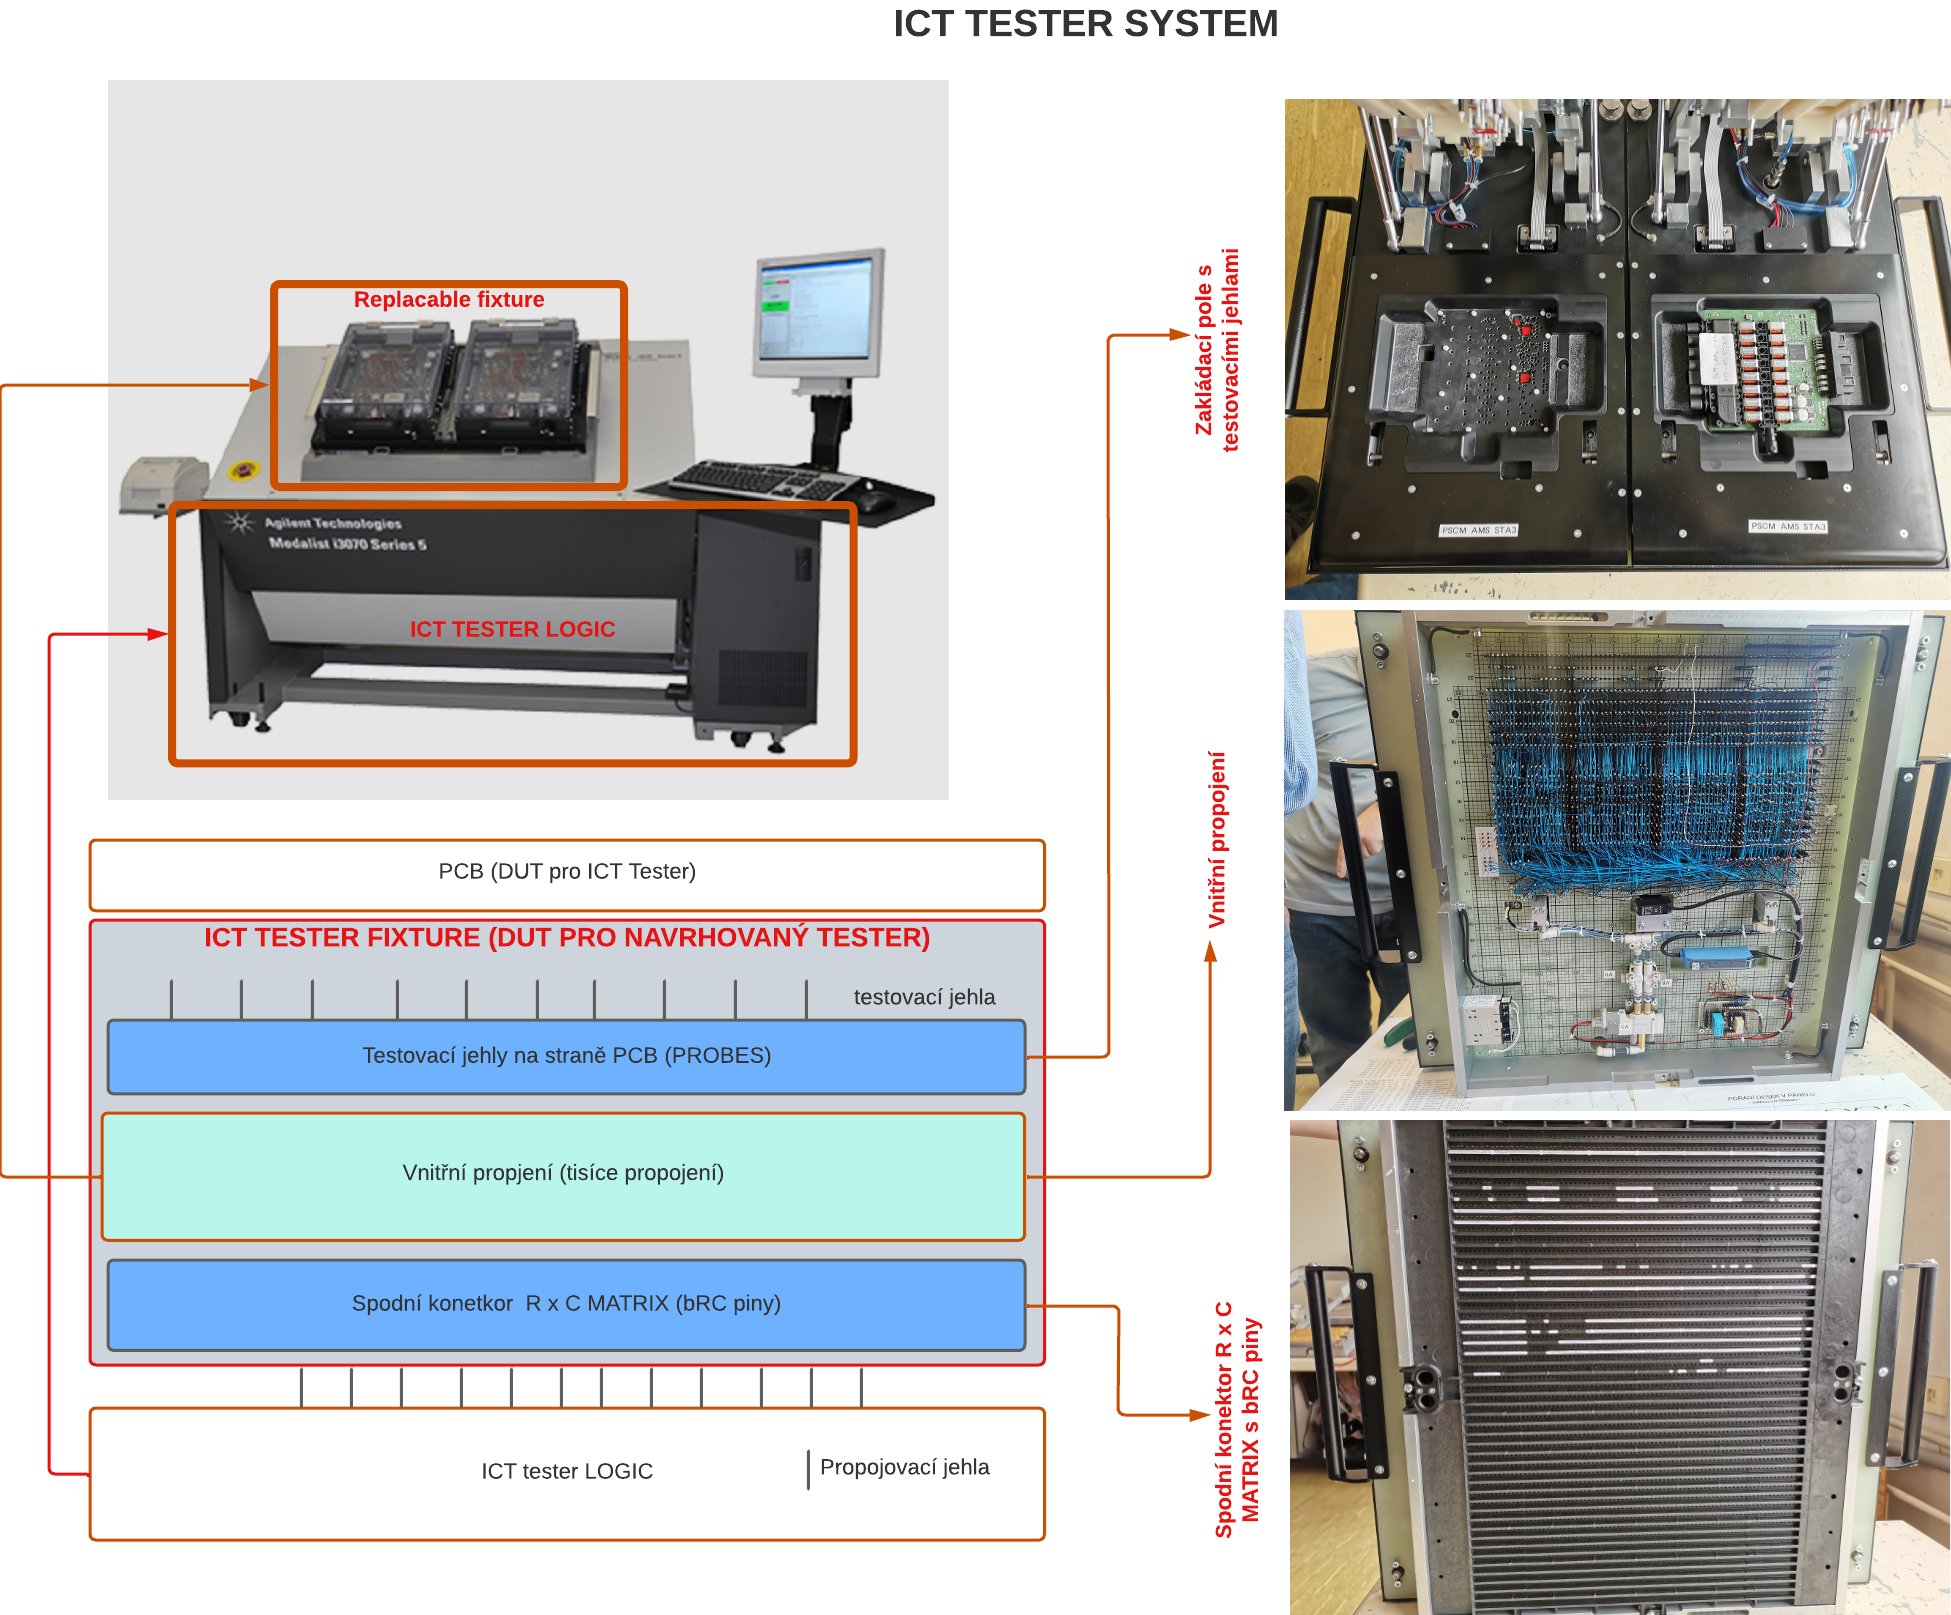
\includegraphics[height = 0.8\textheight]{obrazky/ICT_tester.png}
		\end{minipage}
	\end{figure}
\end{frame}

\begin{frame} 
	% nadpis snímku
	\frametitle{PASS/FAIL VS měření přesného odporu}
	\vspace*{1.5cm}
	\begin{table}[ht!]
		\resizebox{\textwidth}{!}{%
		\begin{tabular}{|lccccc|}
		\hline
		\multicolumn{6}{|c|}{\textbf{Požadované charekteristiky měřícího obvodu}}                                                                                                                                                                                                                                                                                  \\ \hline
		\multicolumn{1}{|l|}{\textbf{TEST MODE}}                & \multicolumn{1}{c|}{\textbf{Počet pinů}} & \multicolumn{1}{c|}{\textbf{Rozsah $[\Omega]$}}  & \multicolumn{1}{c|}{\textbf{Přesnost $[\pm \Omega]$}} & \multicolumn{1}{c|}{\textbf{čas $[\mu s/pin]$}} & \textbf{Celkový čas $[ms]$} \\ \hline
		\multicolumn{1}{|l|}{\textbf{PASS/FAIL}}                & \multicolumn{1}{c|}{4000}                & \multicolumn{1}{c|}{1-101}                      & \multicolumn{1}{c|}{3}                                & \multicolumn{1}{c|}{2,5}                        & 10                          \\ \hline
		\multicolumn{1}{|l|}{\textbf{PASS/FAIL}}                & \multicolumn{1}{c|}{4000}                & \multicolumn{1}{c|}{101-1000}                      & \multicolumn{1}{c|}{rel. chyba 5\%}                                & \multicolumn{1}{c|}{2,5}                        & 10                          \\ \hline
		\multicolumn{1}{|l|}{\textbf{Měření   "pravé"\ hodnoty}} & \multicolumn{1}{c|}{4000}                & \multicolumn{1}{c|}{1-101}                      & \multicolumn{1}{c|}{3}                                & \multicolumn{1}{c|}{Nedefinován}                & Nedefinován                 \\ \hline
		\multicolumn{1}{|l|}{\textbf{Měření   "pravé"\ hodnoty}} & \multicolumn{1}{c|}{4000}                & \multicolumn{1}{c|}{101-1000}                      & \multicolumn{1}{c|}{rel. chyba 5\%}                                & \multicolumn{1}{c|}{Nedefinován}                & Nedefinován                 \\ \hline
		\end{tabular}%
		}
		\caption{Požadované měřící charakteristiky}
		\label{tab:Požadované měřící charakteristiky}
	\end{table}
\end{frame}

\begin{frame} 
	% nadpis snímku
	\frametitle{Koncepce měření 1/3}
	\vspace*{0.5cm}
	\begin{figure}[ht!]
		\centering
		%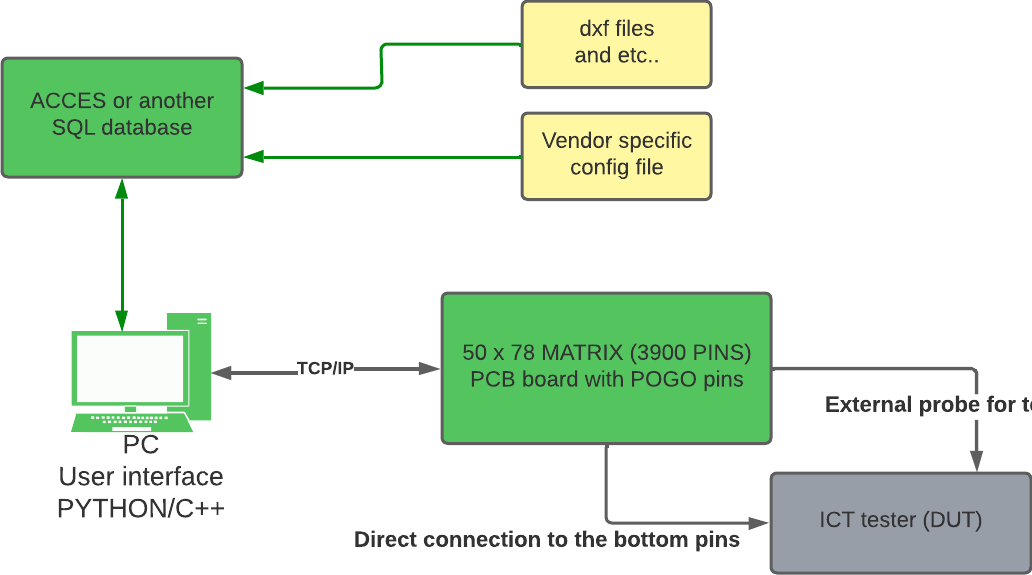
\includegraphics[width = \textwidth]{obrazky/system_connection.png}
		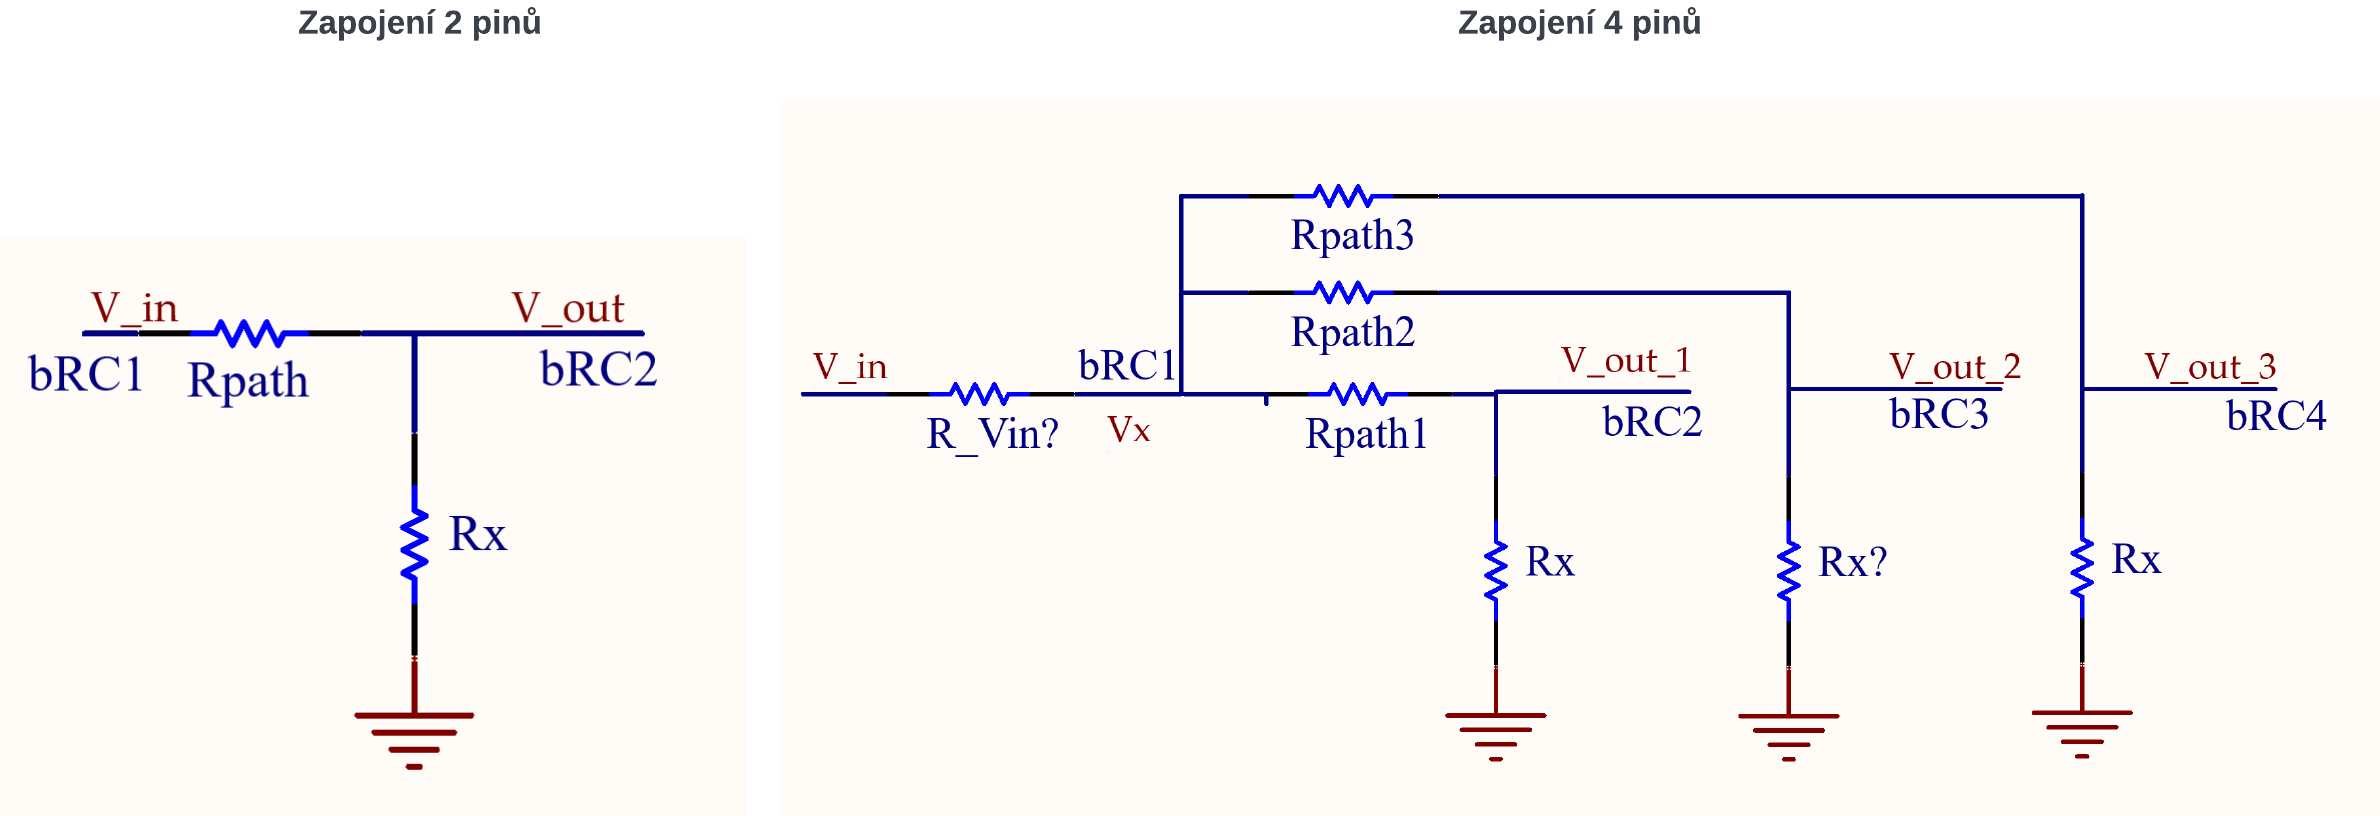
\includegraphics[width = \textwidth]{obrazky/2_and_4_pins_connection.png}
	\end{figure}
\end{frame}

\begin{frame} 
	% nadpis snímku
	\frametitle{Koncepce měření 2/3}
	\vspace*{0.5cm}
	\begin{figure}[ht!]
		\centering
		%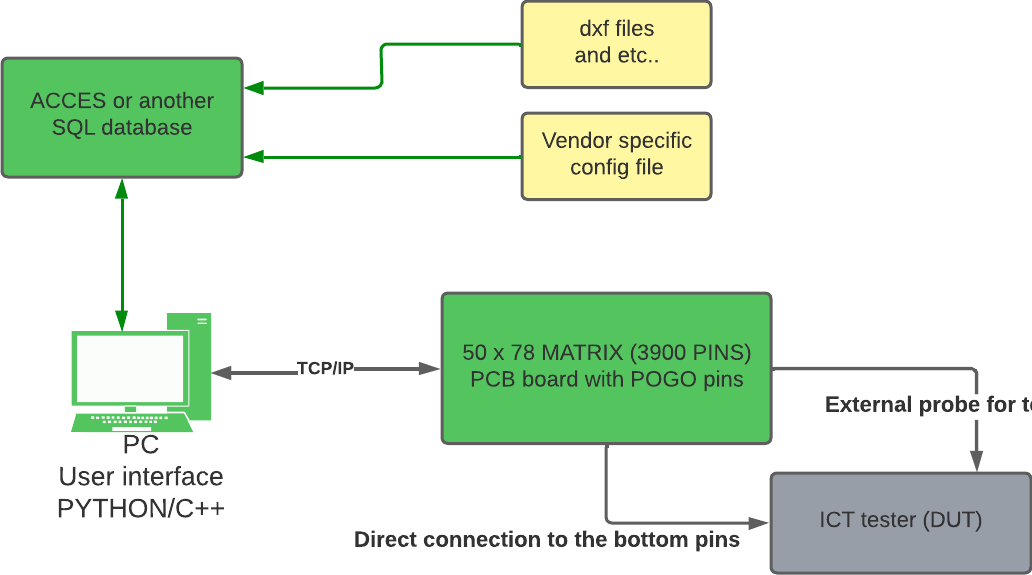
\includegraphics[width = \textwidth]{obrazky/system_connection.png}
		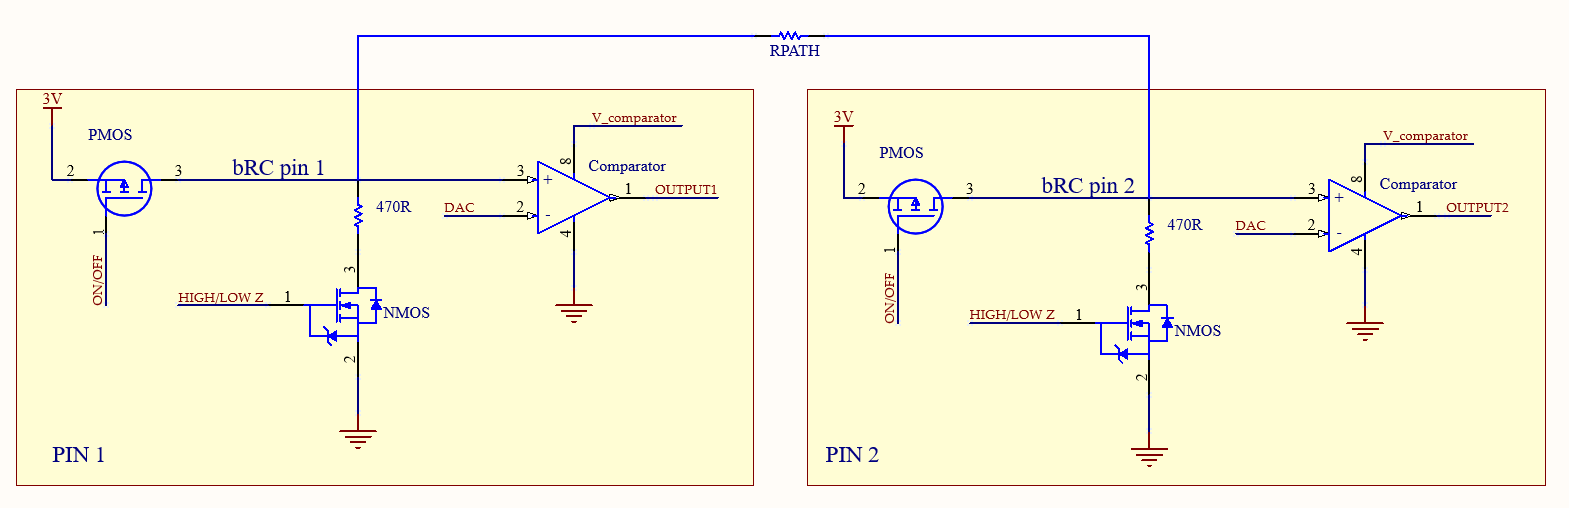
\includegraphics[width = \textwidth]{obrazky/R_meas_obhj.png}
	\end{figure}
\end{frame}

\begin{frame} 
	% nadpis snímku
	\frametitle{Koncepce měření 3/3}
	\vspace*{0.5cm}
	\begin{figure}[ht!]
		\centering
		%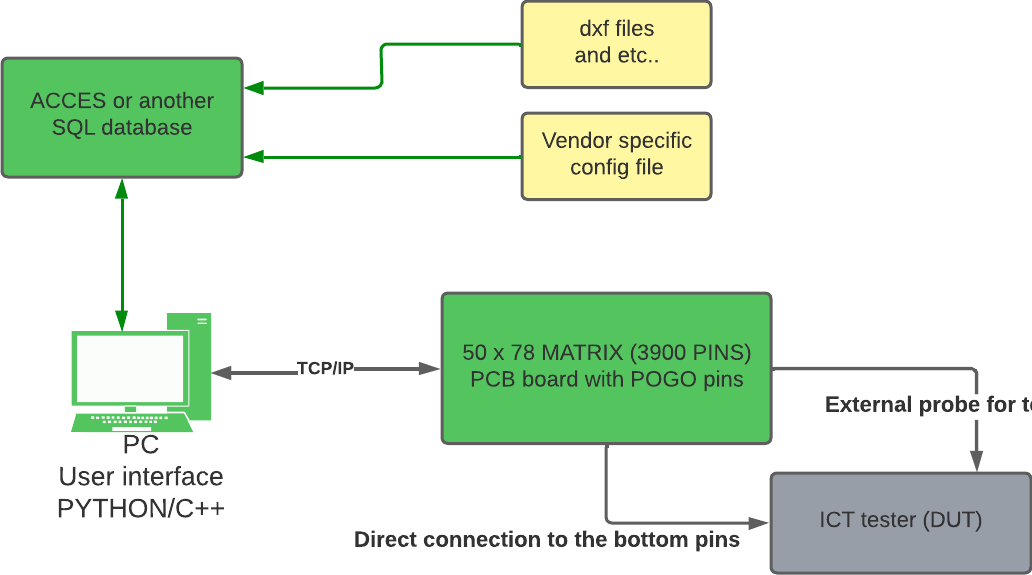
\includegraphics[width = \textwidth]{obrazky/system_connection.png}
		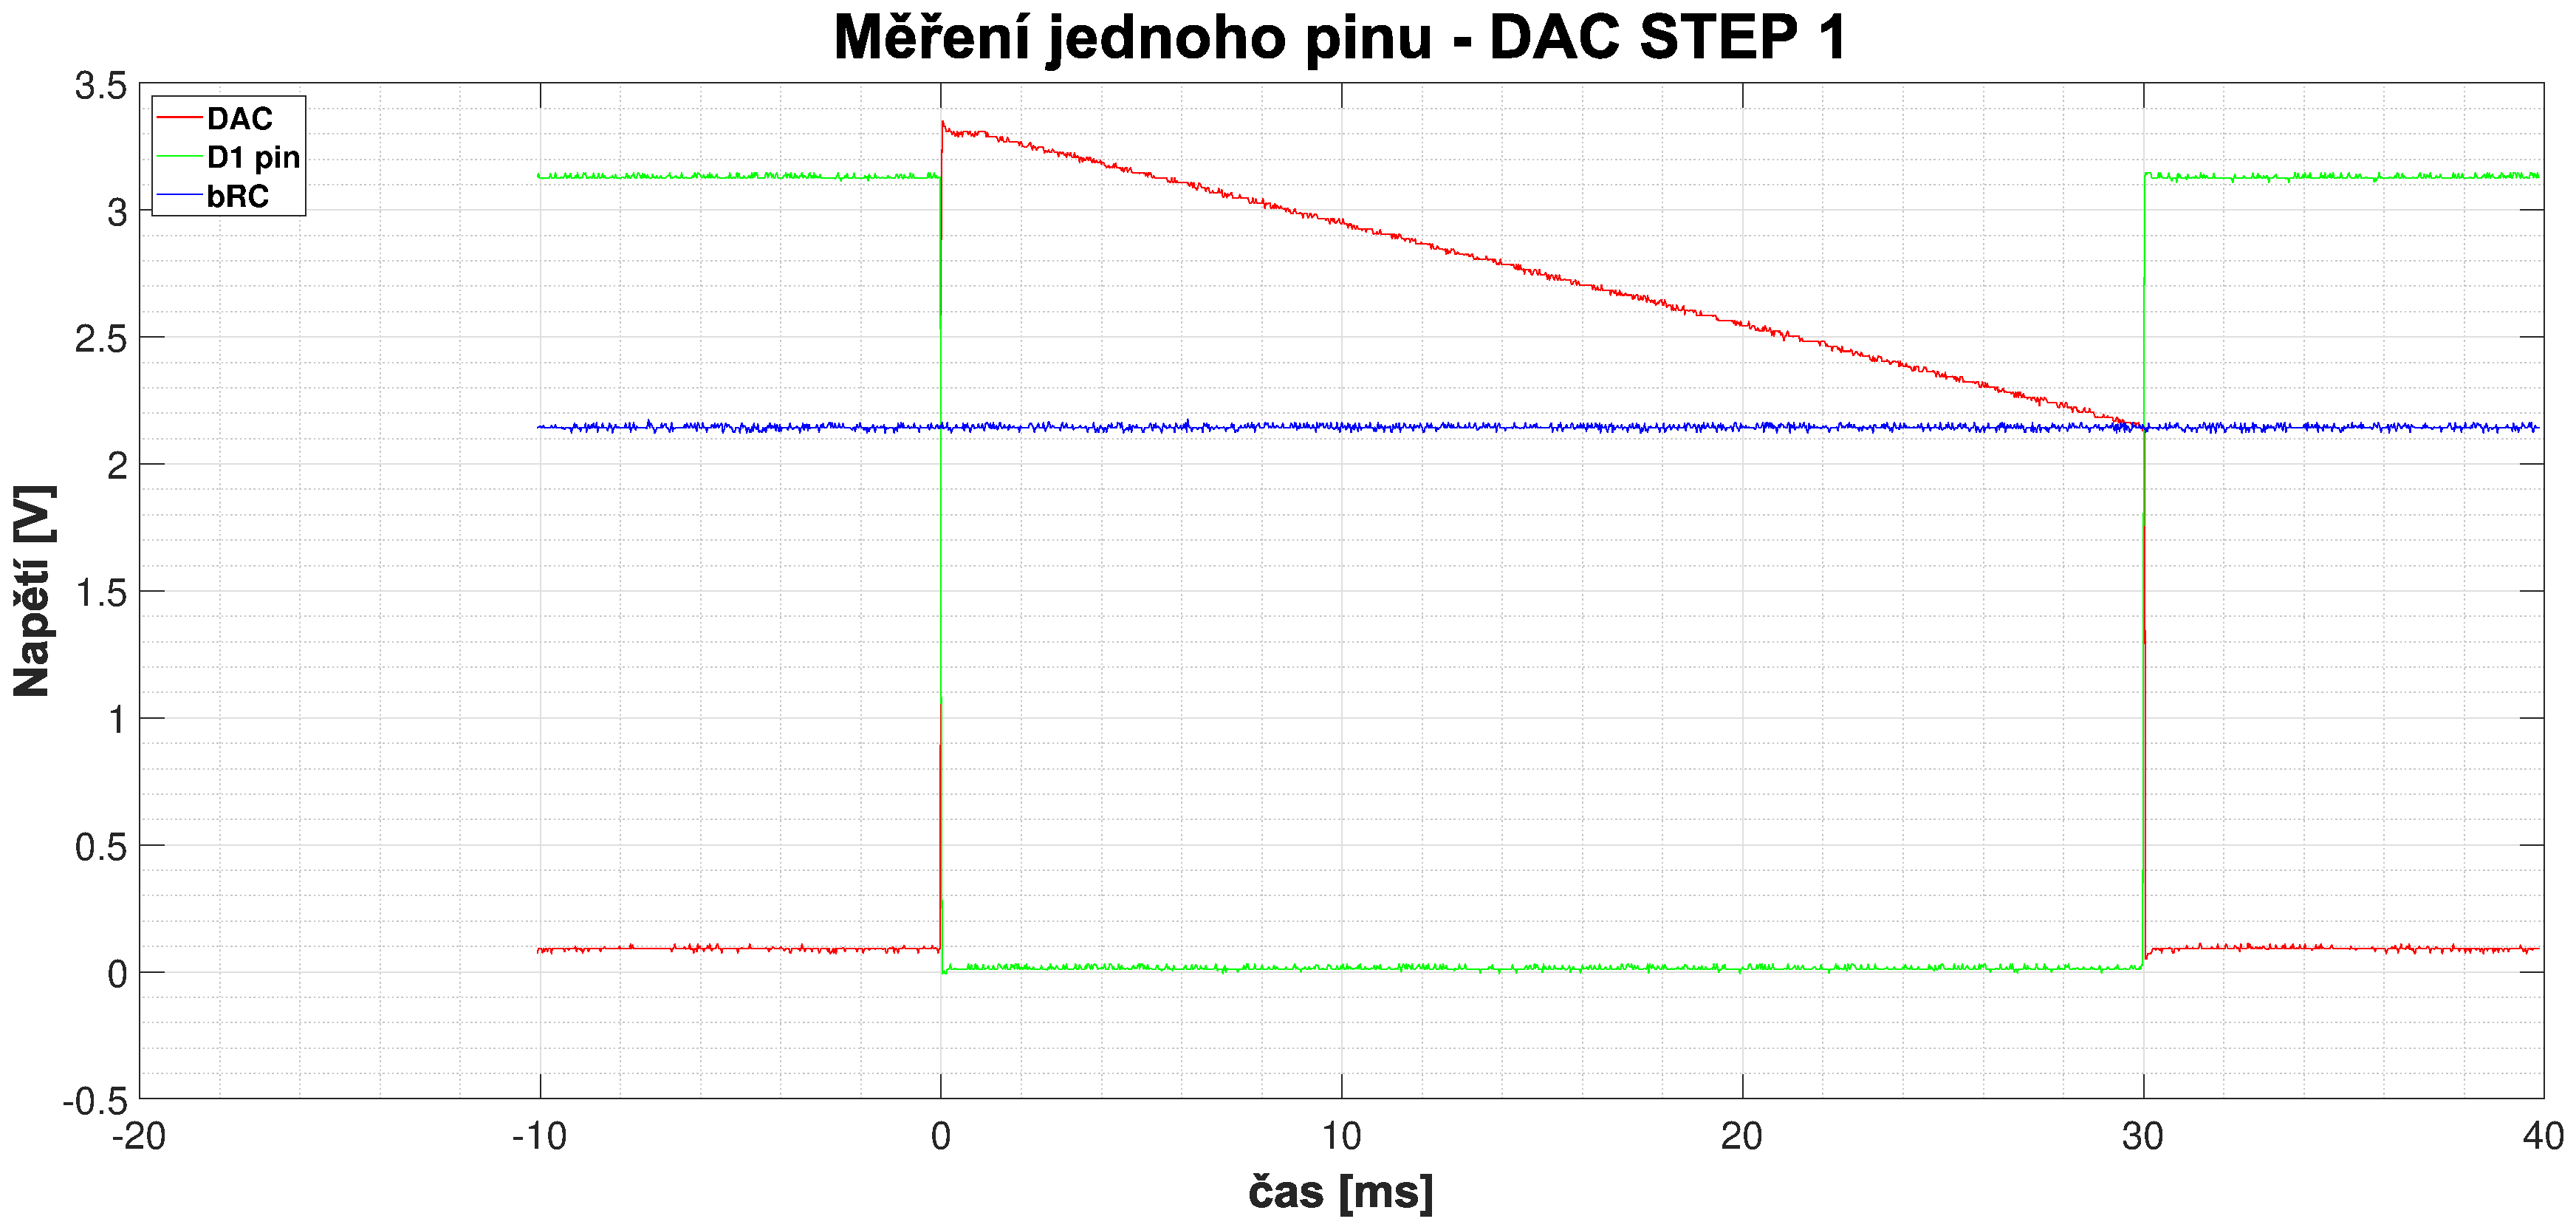
\includegraphics[width = \textwidth]{obrazky/matlab_generated/pin_step1.eps}
	\end{figure}
\end{frame}

\begin{frame} 
	% nadpis snímku
	\frametitle{Koncepce testeru}
	\vspace*{0.5cm}
	\begin{figure}[ht!]
		\centering
		%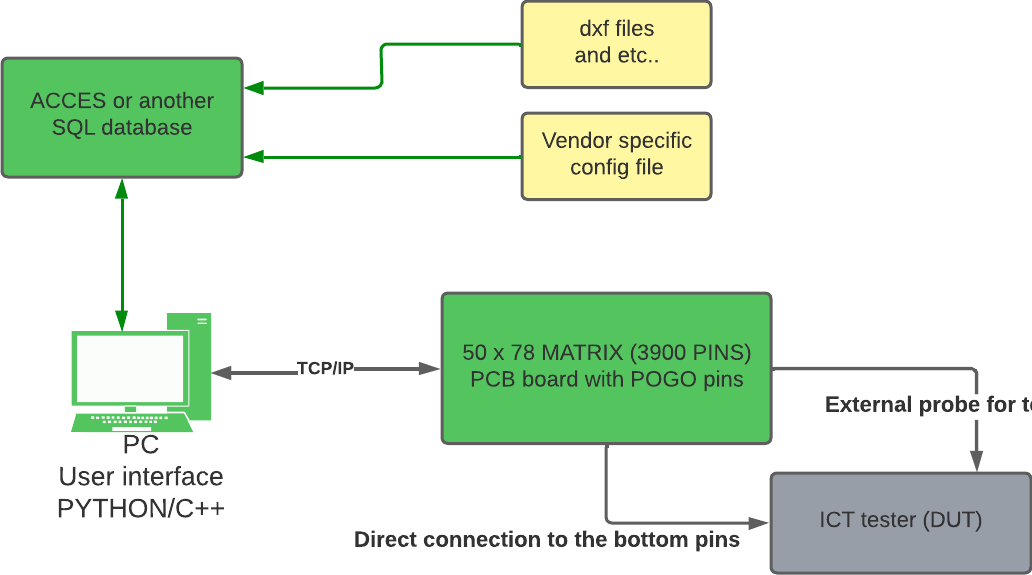
\includegraphics[width = \textwidth]{obrazky/system_connection.png}
		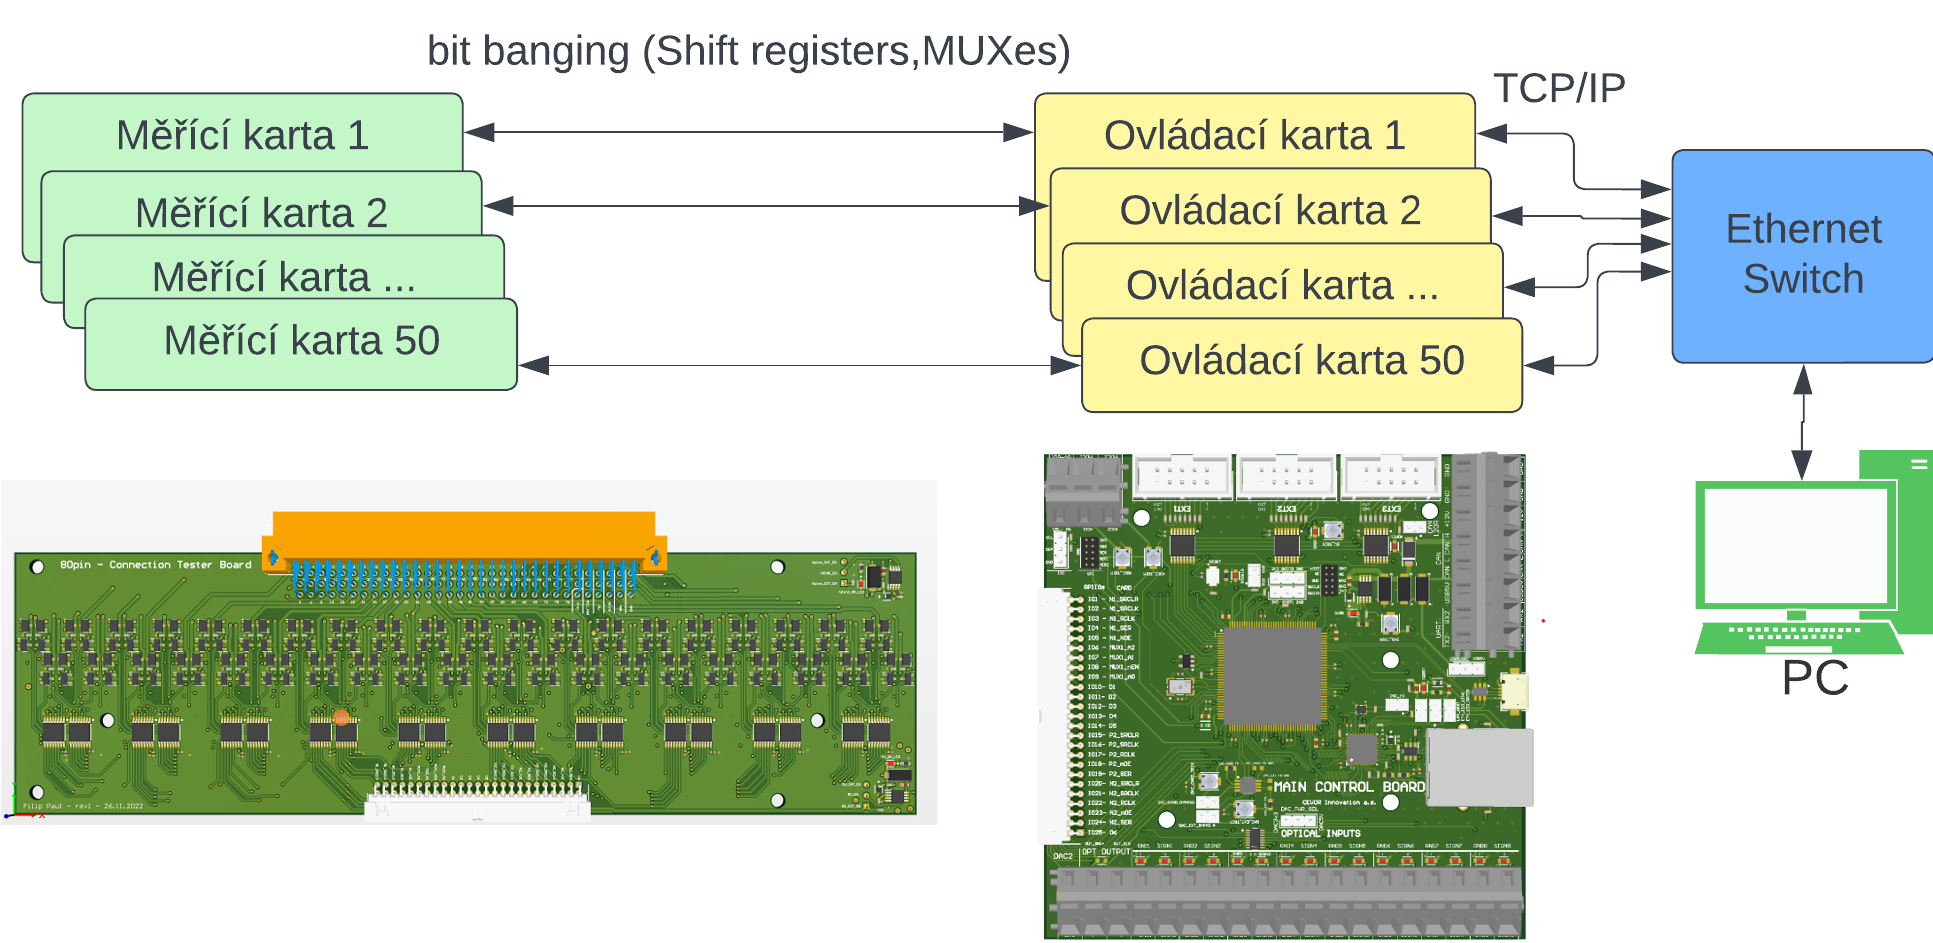
\includegraphics[width = \textwidth]{obrazky/system_karet_obh.png}
	\end{figure}
\end{frame}


\begin{frame} 
	% nadpis snímku
	\frametitle{Foto propojení měřící a ovládací karty}
	\begin{figure}[ht!]
		\centering
		%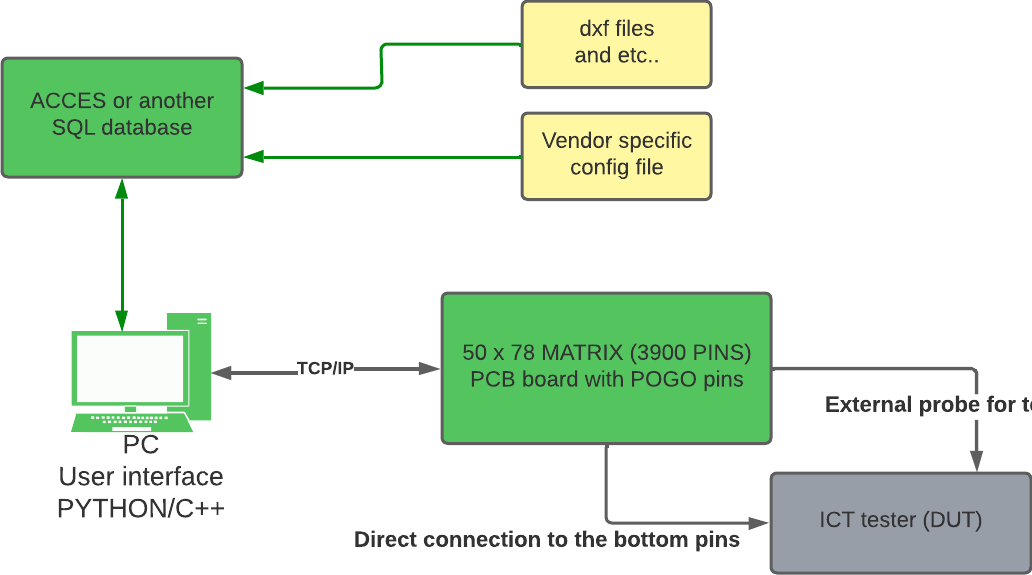
\includegraphics[width = \textwidth]{obrazky/system_connection.png}
		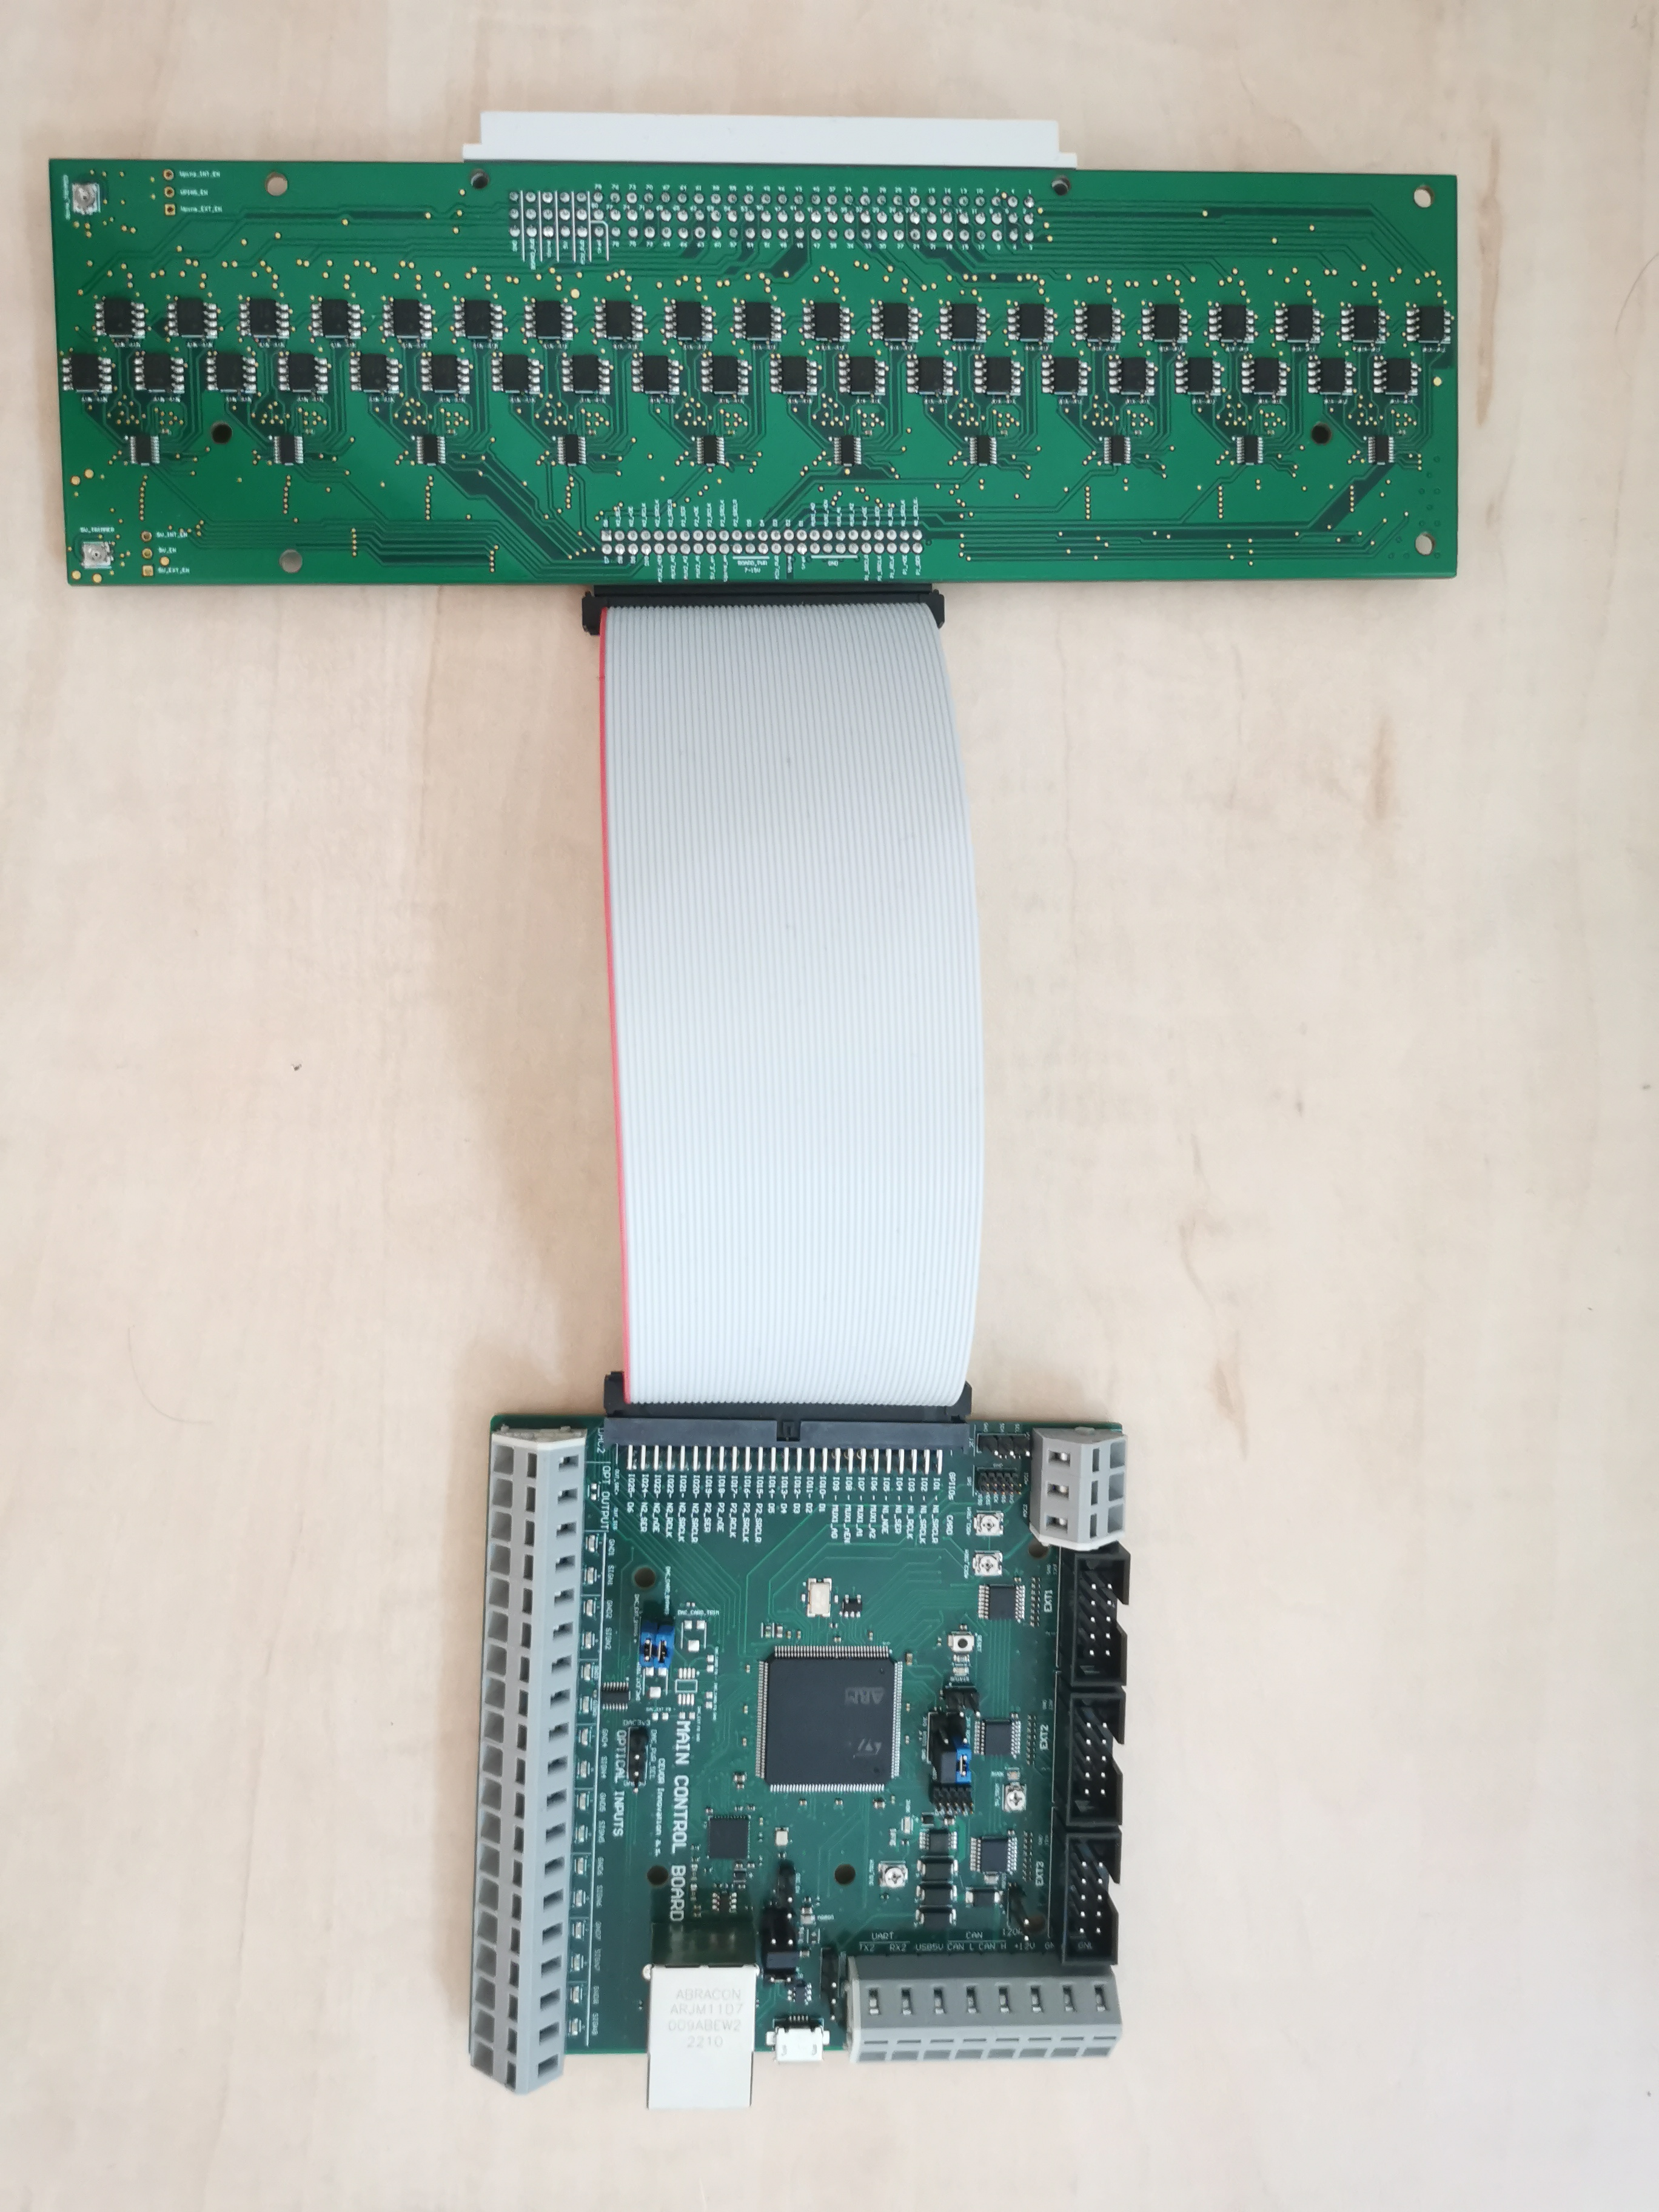
\includegraphics[height = 0.7\textwidth, angle = 90]{obrazky/foto_obh.jpg}
	\end{figure}
\end{frame}

\begin{frame} 
	% nadpis snímku
	\frametitle{Měřící karta 1/2}
	\vspace*{0.5cm}
	\begin{figure}[ht!]
		\centering
		%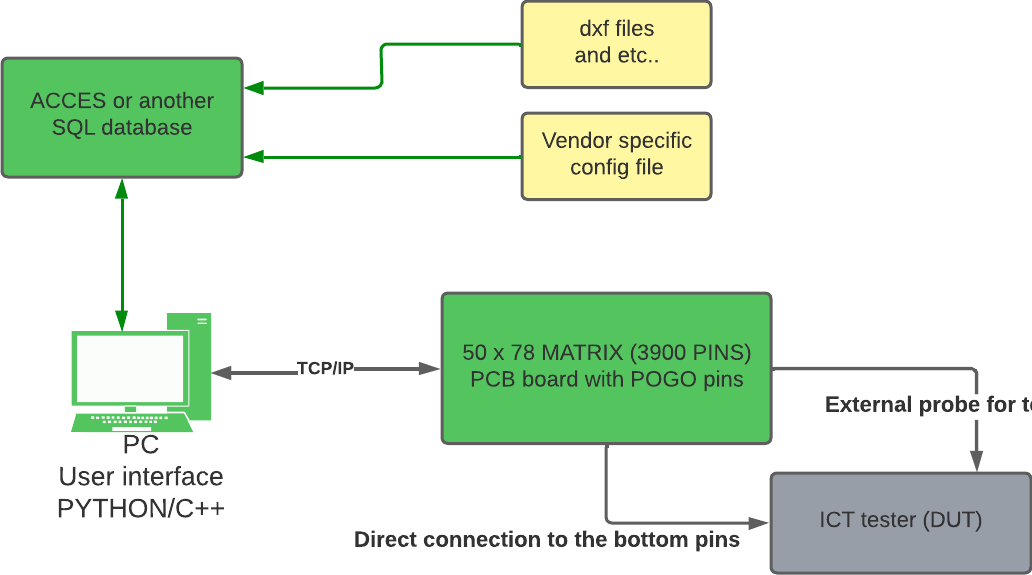
\includegraphics[width = \textwidth]{obrazky/system_connection.png}
		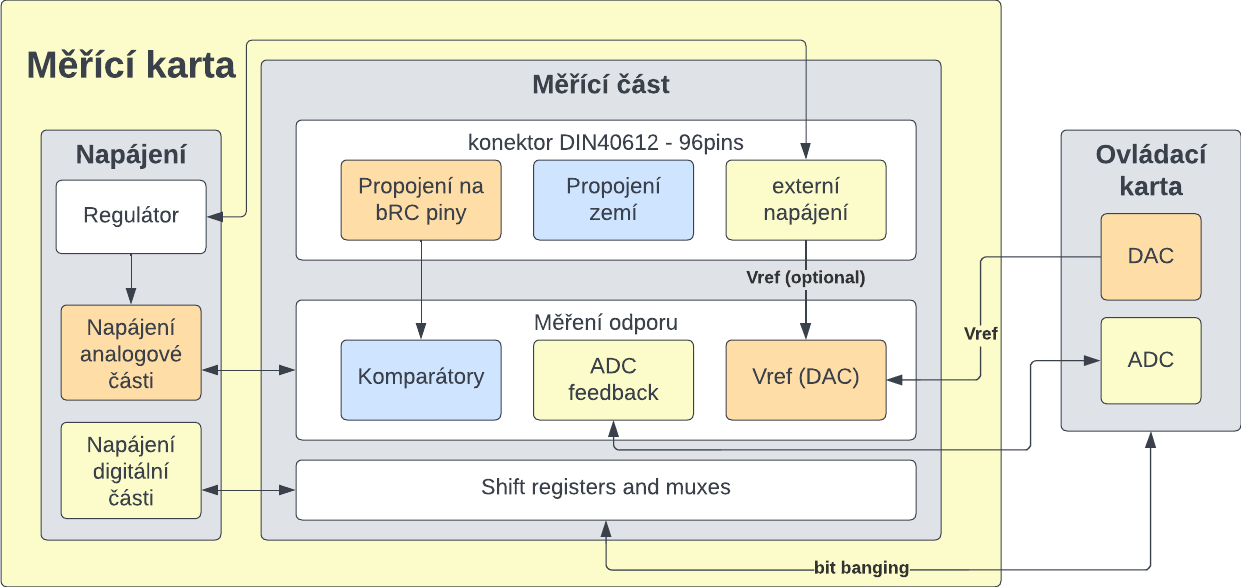
\includegraphics[width = \textwidth]{obrazky/karta_system_diagram.png}
	\end{figure}
\end{frame}

\begin{frame} 
	% nadpis snímku
	\frametitle{Měřící karta  2/2}
	\vspace*{1cm}
	\begin{figure}[ht!]
		\centering
		%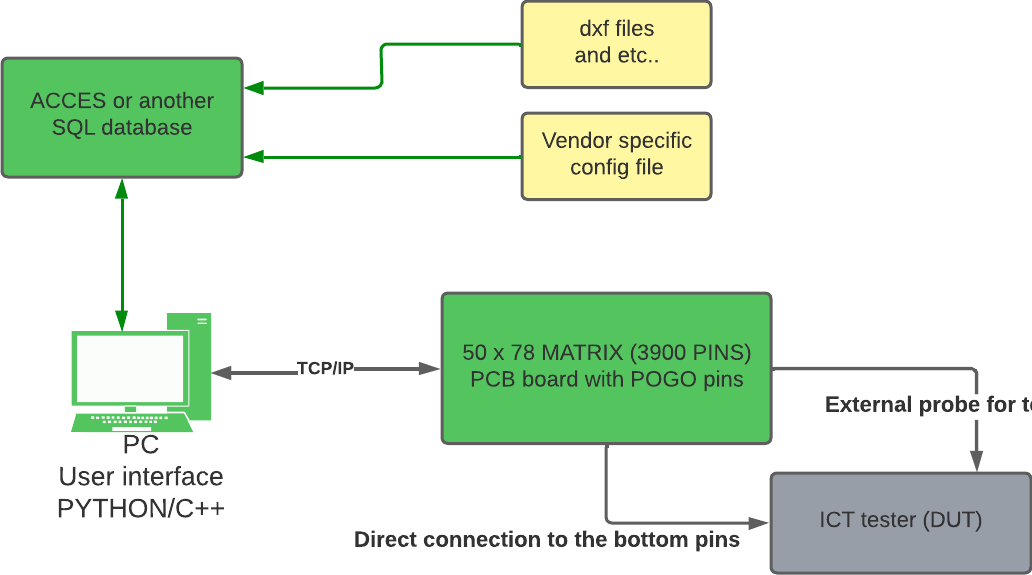
\includegraphics[width = \textwidth]{obrazky/system_connection.png}
		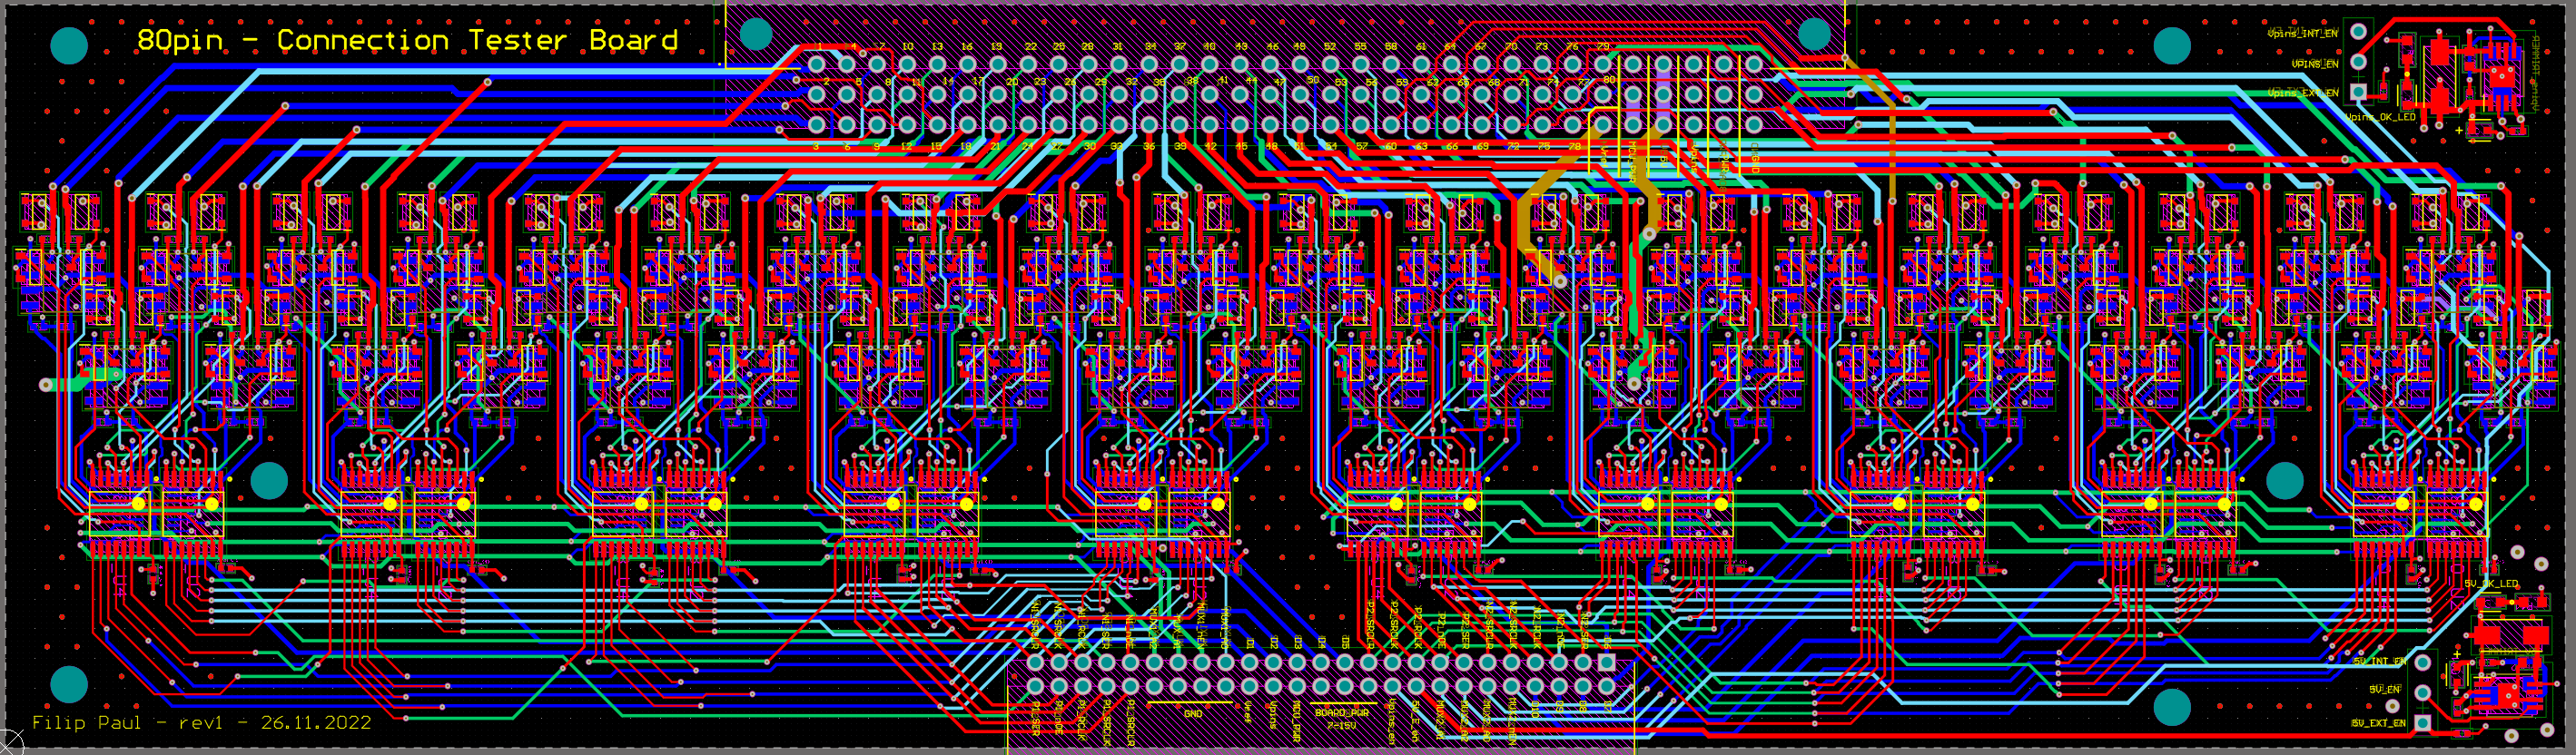
\includegraphics[width = \textwidth]{obrazky/all_layers_no_poly.png}
	\end{figure}
\end{frame}

\begin{frame} 
	% nadpis snímku
	\frametitle{Ovládací karta 1/2}

	\begin{figure}[ht!]
		\centering
		%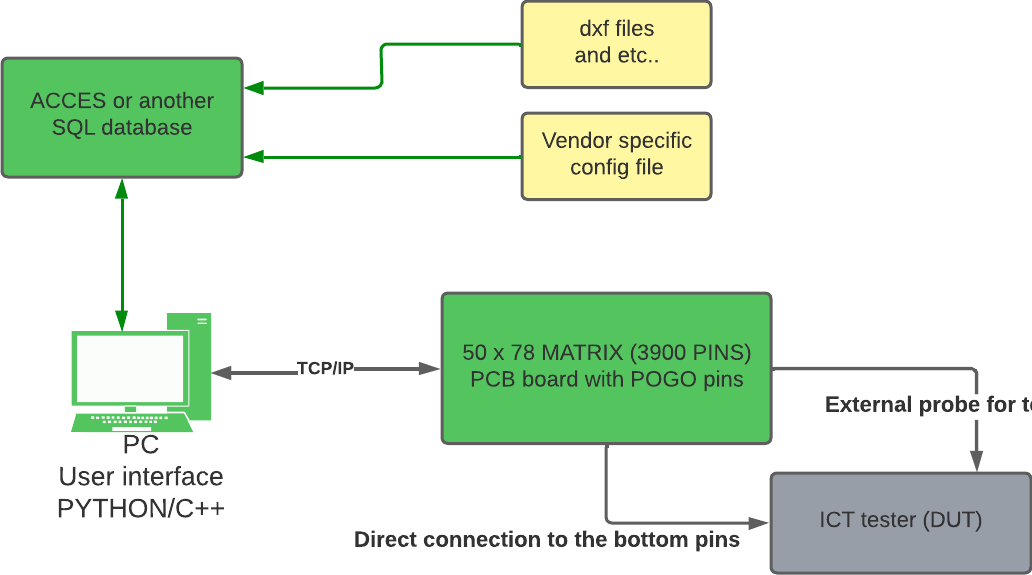
\includegraphics[width = \textwidth]{obrazky/system_connection.png}
		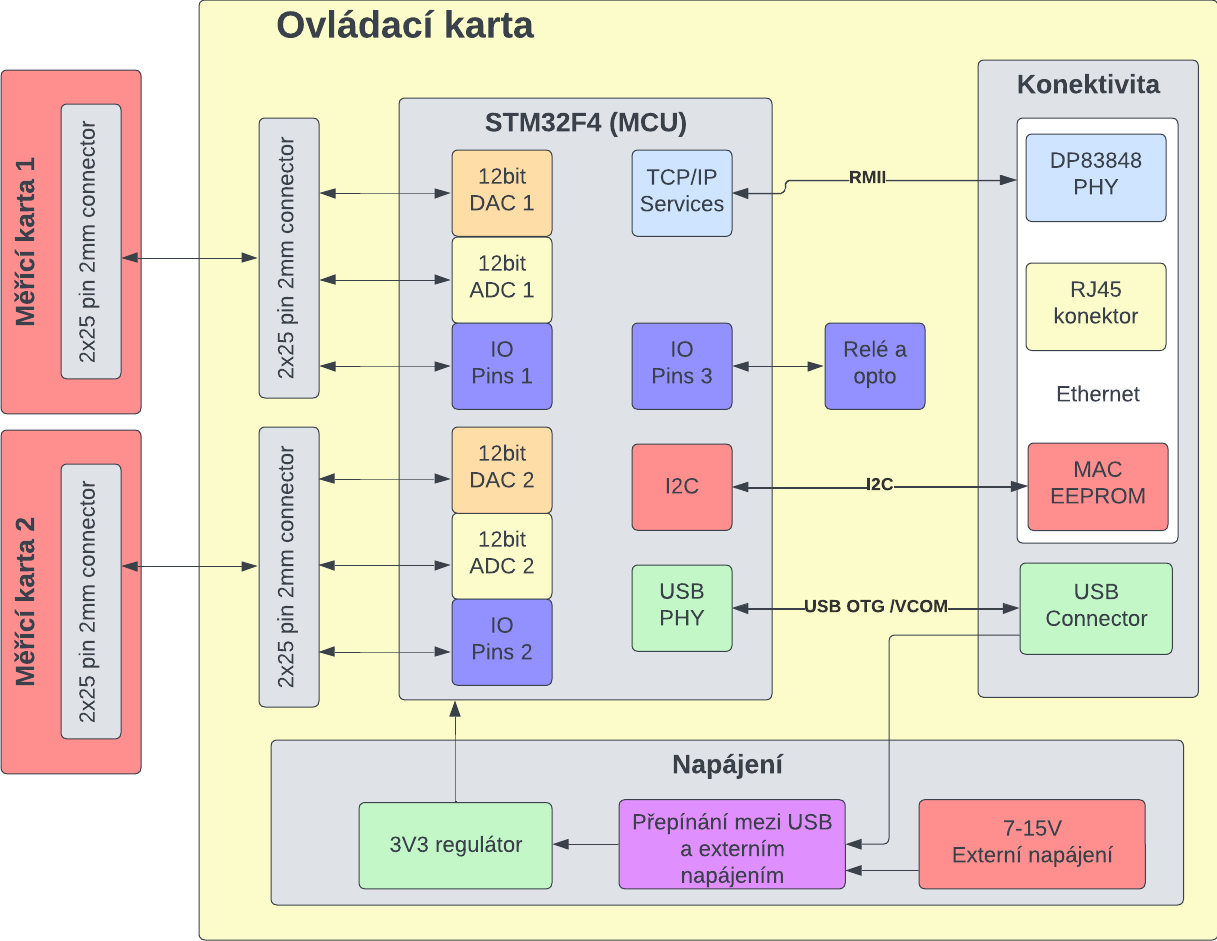
\includegraphics[height = 0.8\textheight]{obrazky/ovladaci_karta_diag.png}
	\end{figure}
\end{frame}

\begin{frame} 
	% nadpis snímku
	\frametitle{Ovládací karta 2/2}

	\begin{figure}[ht!]
		\centering
		%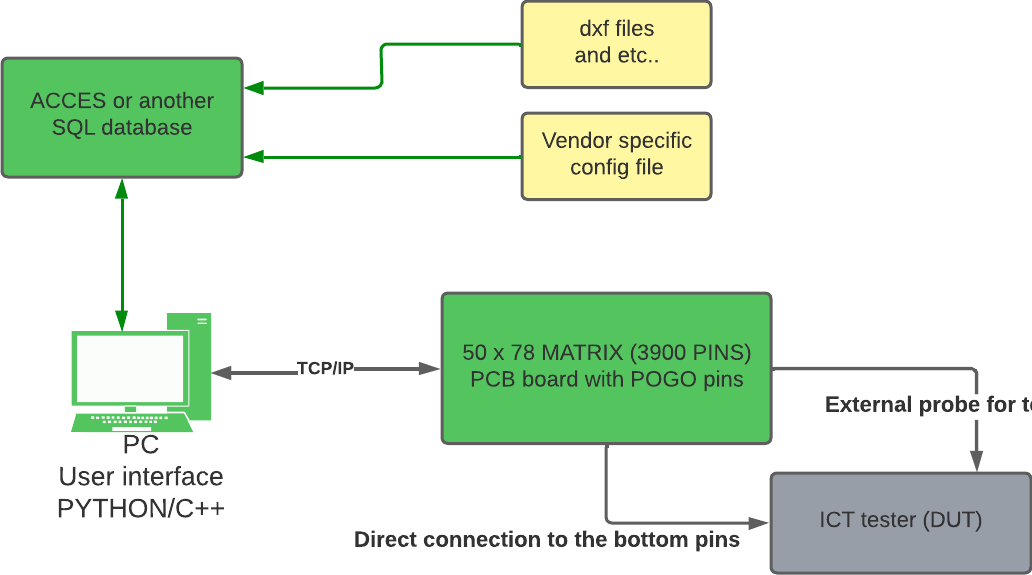
\includegraphics[width = \textwidth]{obrazky/system_connection.png}
		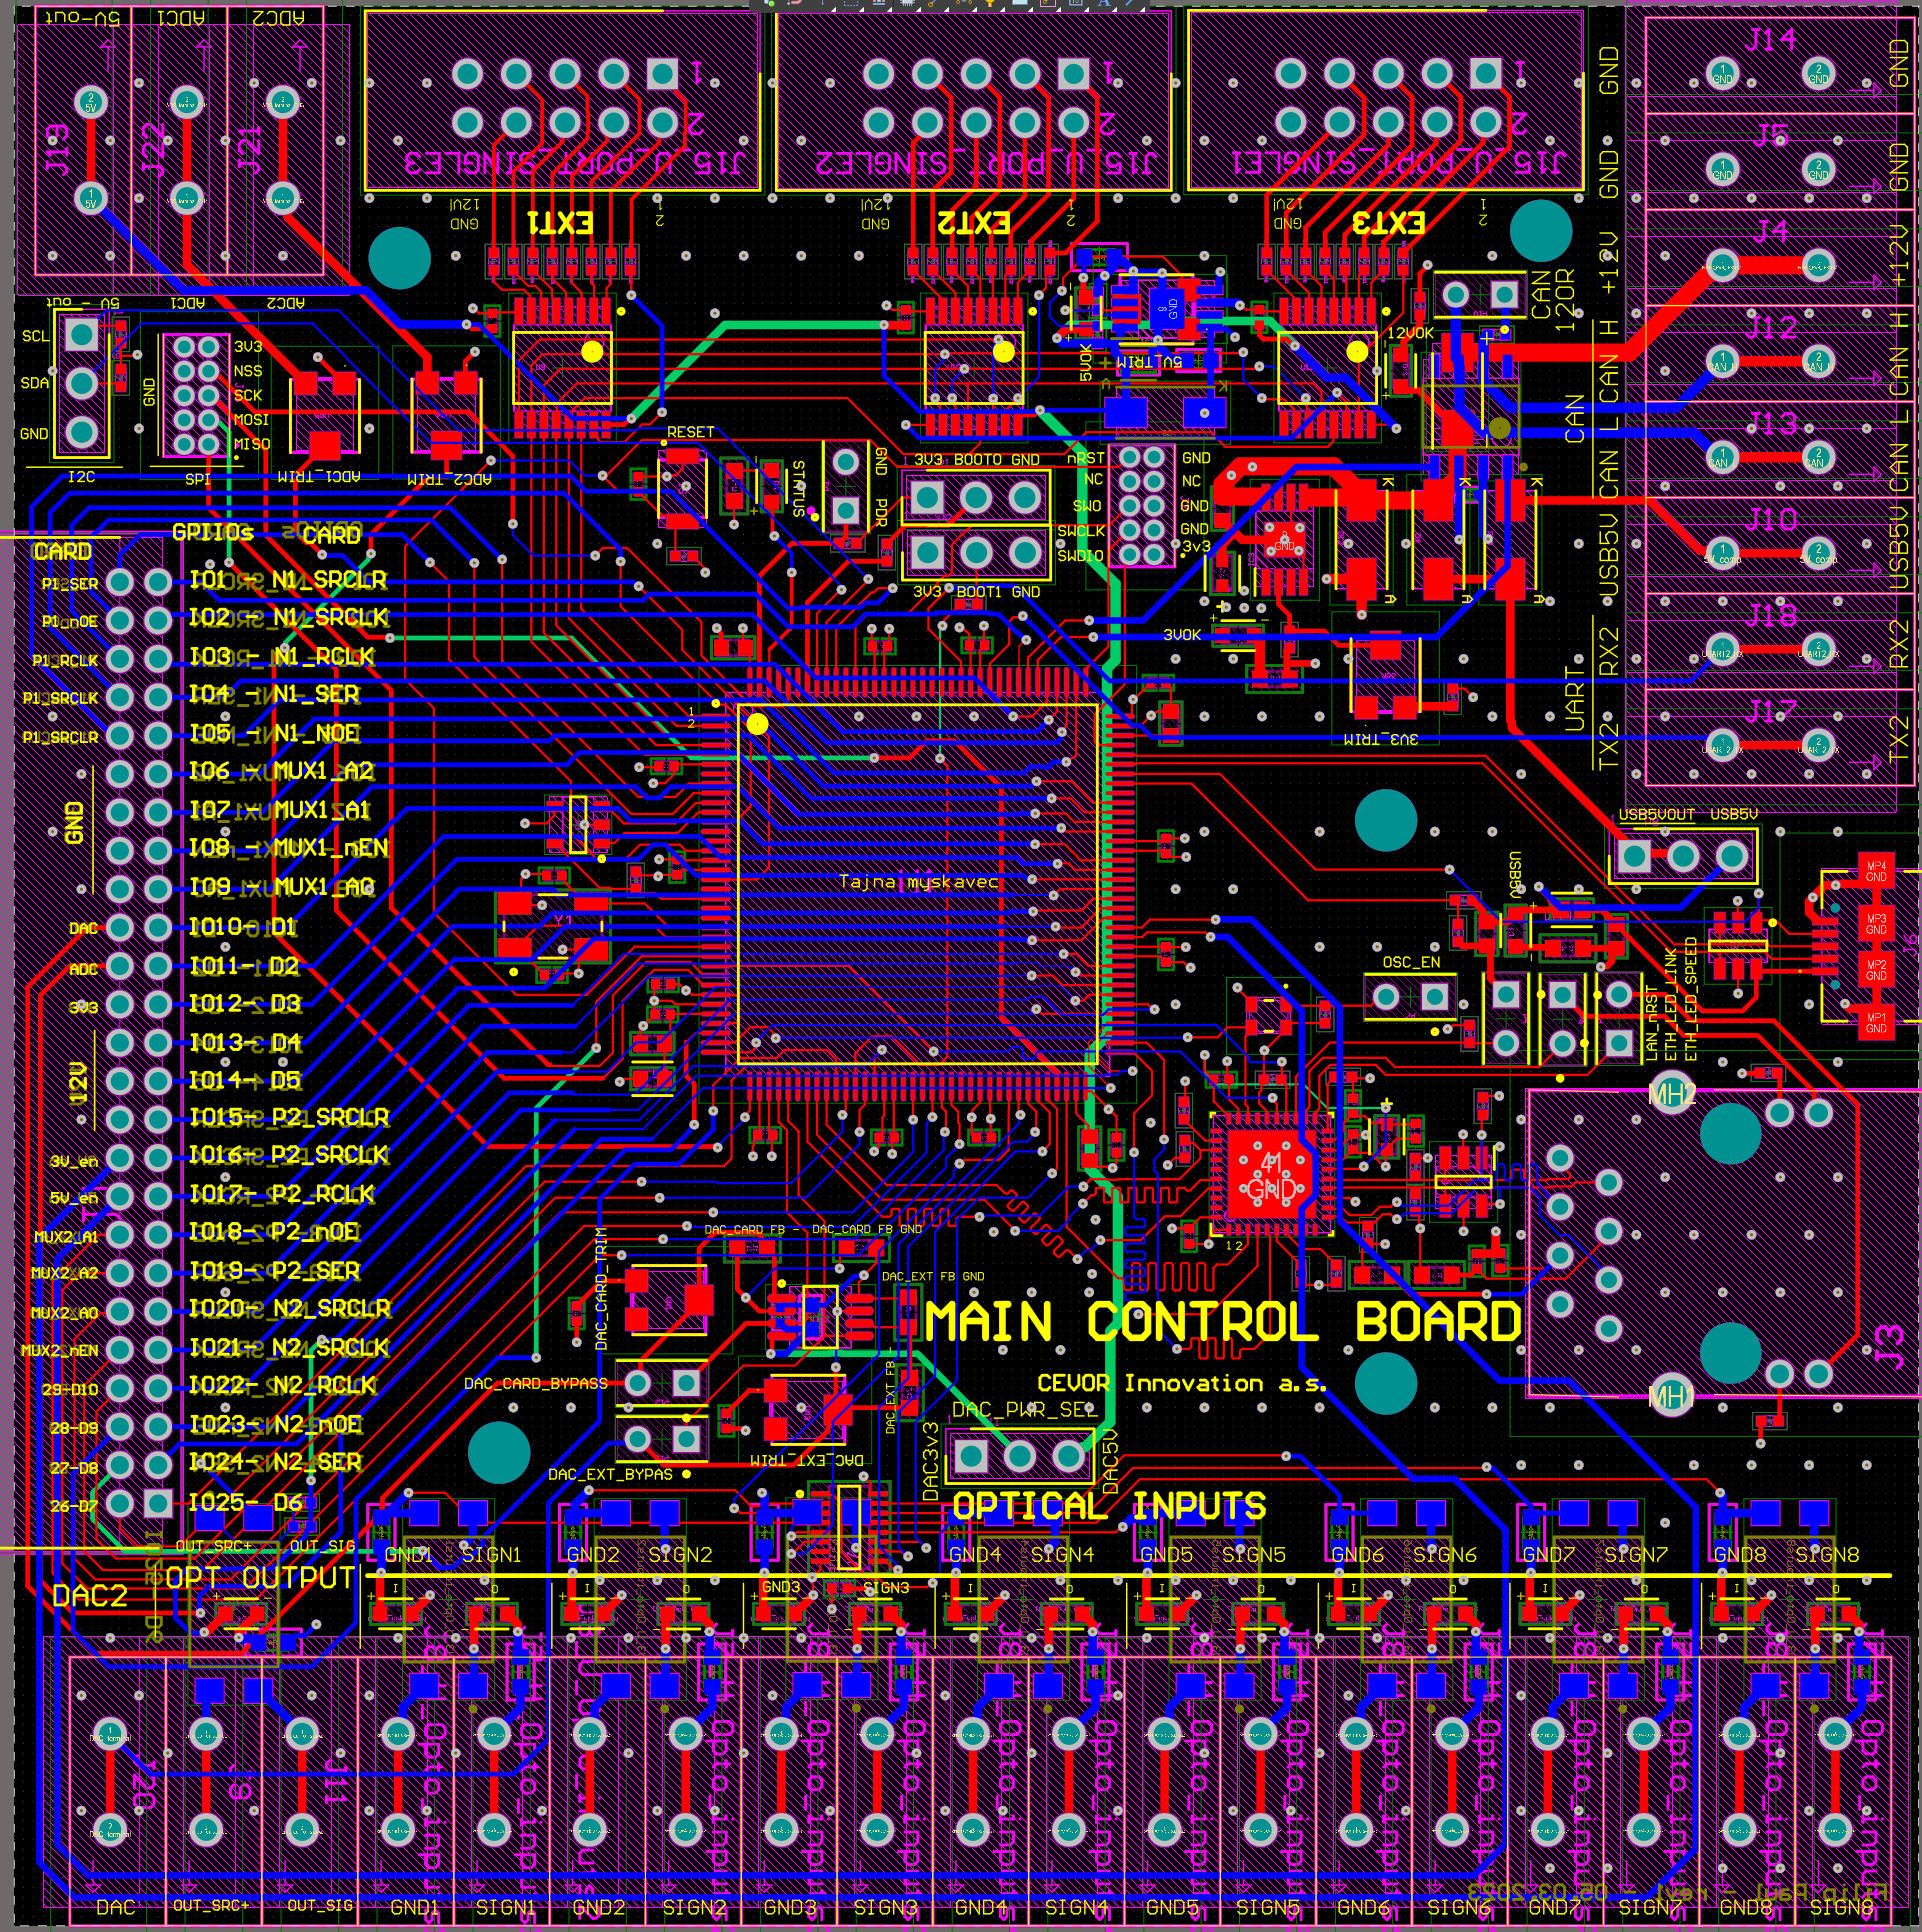
\includegraphics[height = 0.8\textheight]{obrazky/all_layers_no_poly_control.png}
	\end{figure}
\end{frame}

\begin{frame} 
	% nadpis snímku
	\frametitle{Dosažená přesnost měření 1/3}

	\begin{figure}[ht!]
		\centering
		%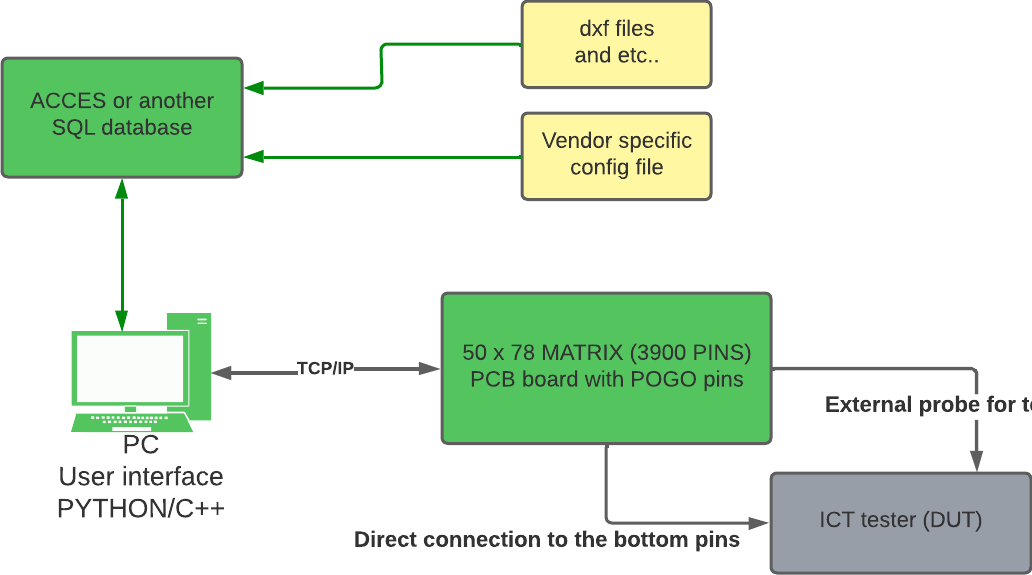
\includegraphics[width = \textwidth]{obrazky/system_connection.png}
		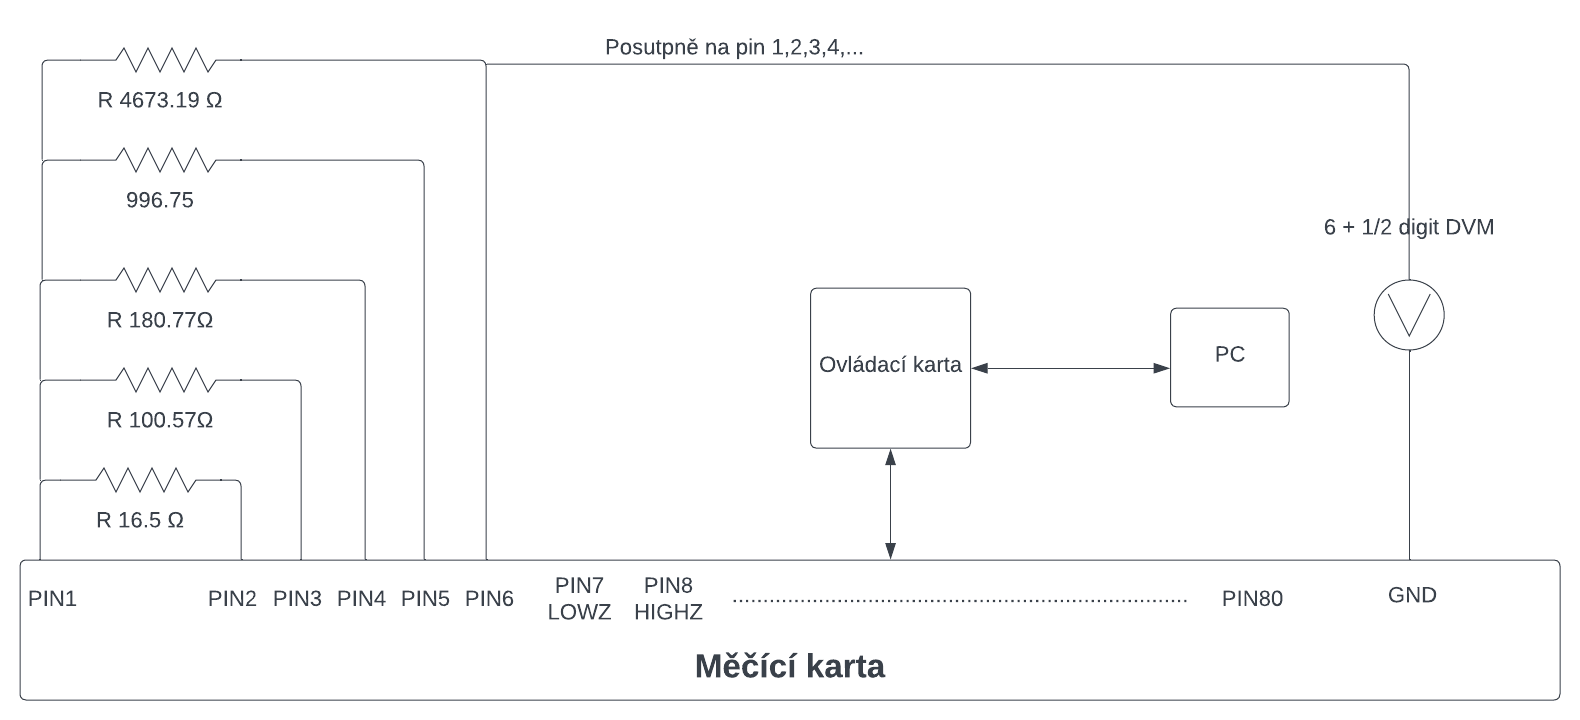
\includegraphics[width = \textwidth]{obrazky/10hourTestScheme.png}
	\end{figure}
\end{frame}

\begin{frame} 
	% nadpis snímku
	\frametitle{Dosažená přesnost měření 2/3}

	\begin{figure}[ht!]
		\centering
		%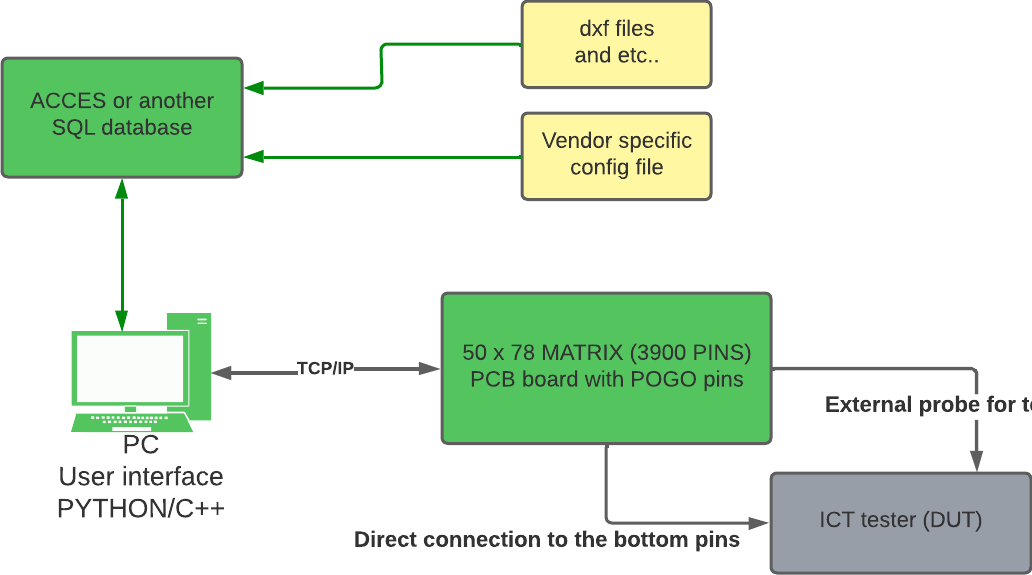
\includegraphics[width = \textwidth]{obrazky/system_connection.png}
		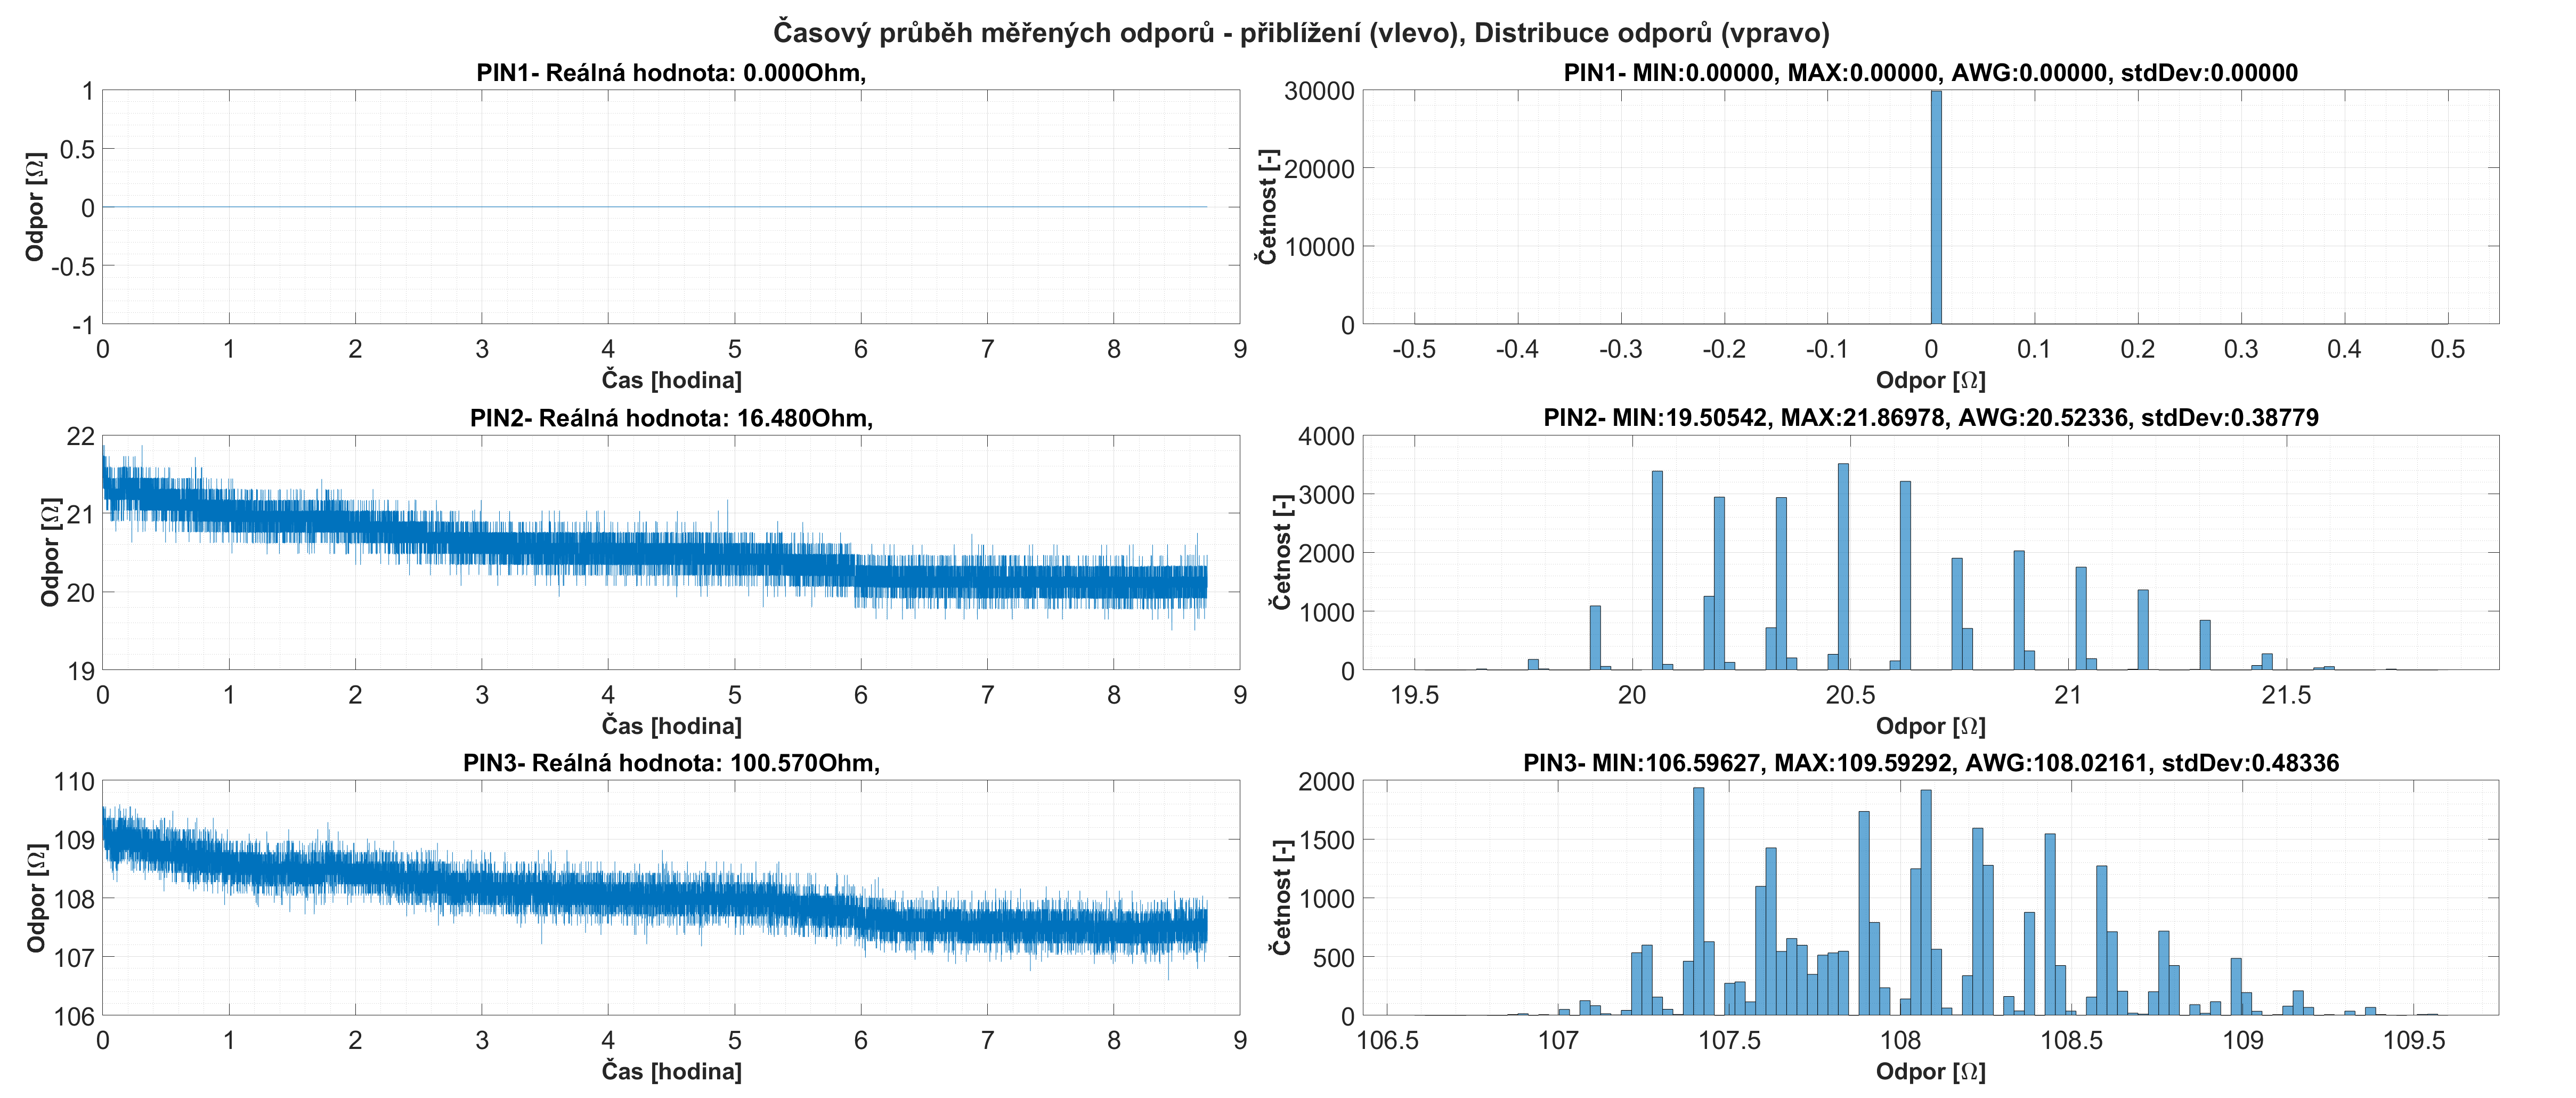
\includegraphics[width = \textwidth]{obrazky/matlab_generated/VOLTAGE_TESTER/dlouhodoba_stabilita_resistor_part1_obhj.eps}
	\end{figure}
\end{frame}

\begin{frame} 
	% nadpis snímku
	\frametitle{Dosažená přesnost a rychlost měření 3/3}
	\vspace*{0.7cm}
	\begin{table}[ht!]
	\centering
		\resizebox{0.7\textwidth}{!}{%
		\begin{tabular}{|l|l|l|l|l|l|}
		\hline
		-        & \textbf{PIN2} & \textbf{PIN3} & \textbf{PIN4} & \textbf{PIN5} & \textbf{PIN6} \\ \hline
		\textbf{ref odpor {[}$\Omega${]}}  & 16.5     & 100.57     & 180.77     & 996.75      & 4673.19 \\ \hline
		\textbf{abs chyba {[}$\Omega${]}}  & 0.11     & 0.62      & 2.15     & 17.61      & 34.42     \\ \hline
		\textbf{rel chyba {[}\%{]}} & 0.647      & 0.616      & 1.189      & 1.767      & 0.737      \\ \hline
		\end{tabular}%
		}
		\caption{Chyby měření odporů vůči pinu č. 1}
		\label{tab:chyby mereni calibrated}
	\end{table}

	\begin{itemize}
		\item Čas měření v PASS/FAIL režimu je závislý převážně na rychlosti zpracování PC aplikace. Obvyklá odezva aplikace je do 50ms.
	\end{itemize}
\end{frame}





\begin{frame} 
	% nadpis snímku
	\frametitle{PC aplikace 1/2}

	\begin{figure}[ht!]
		\centering
		%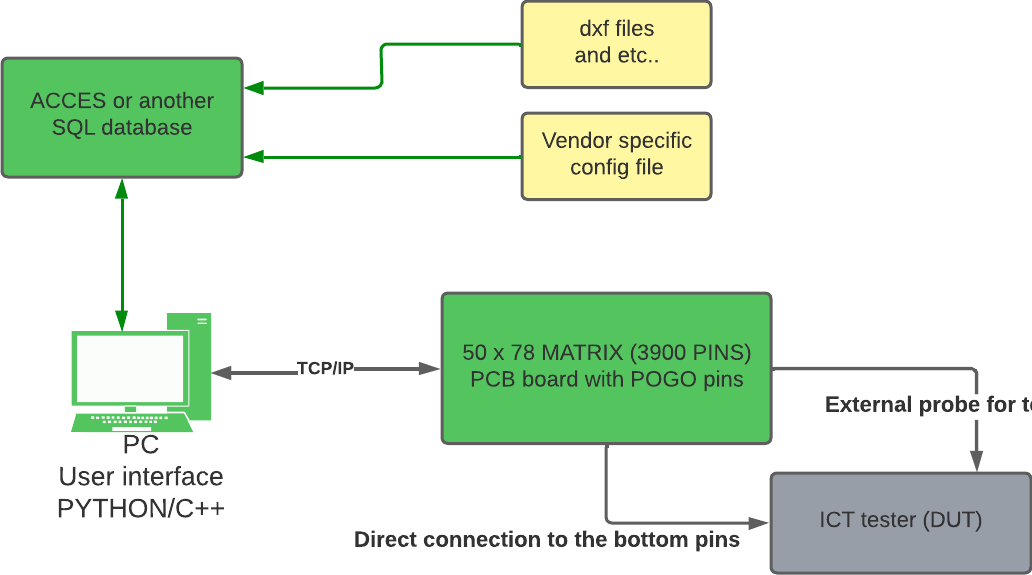
\includegraphics[width = \textwidth]{obrazky/system_connection.png}
		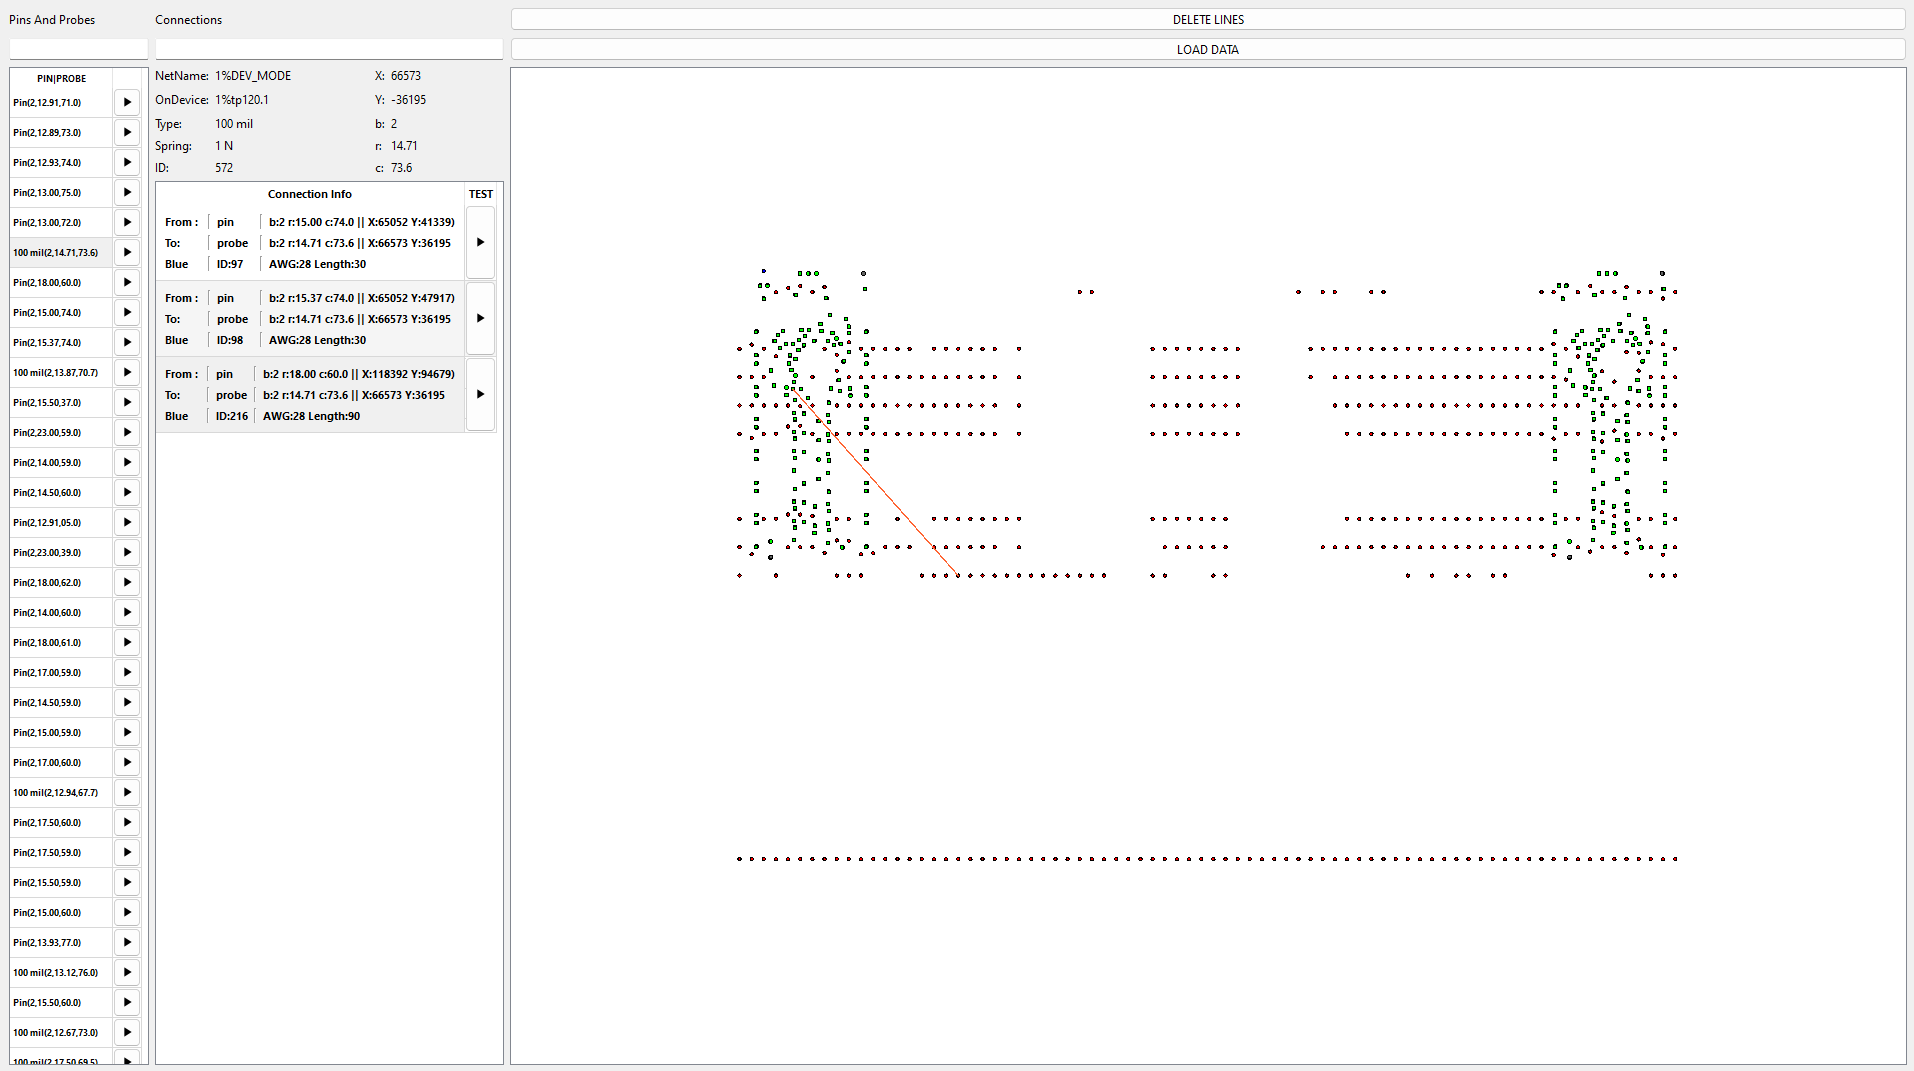
\includegraphics[width = 1\textwidth]{obrazky/PC_APP_dataViewer.png}
	\end{figure}
\end{frame}

\begin{frame} 
	% nadpis snímku
	\frametitle{PC aplikace 2/2}

	\begin{figure}[ht!]
		\centering
		%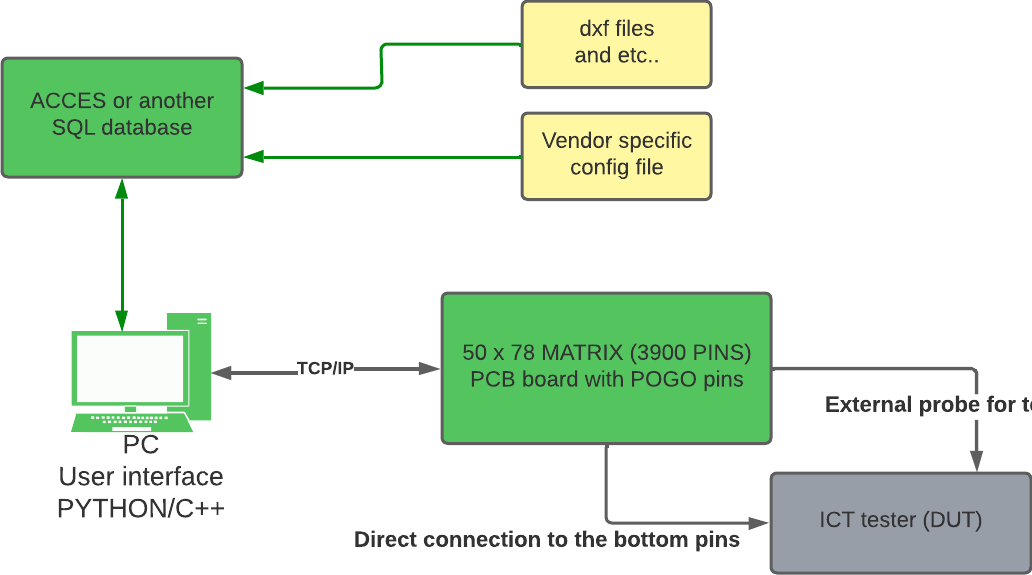
\includegraphics[width = \textwidth]{obrazky/system_connection.png}
		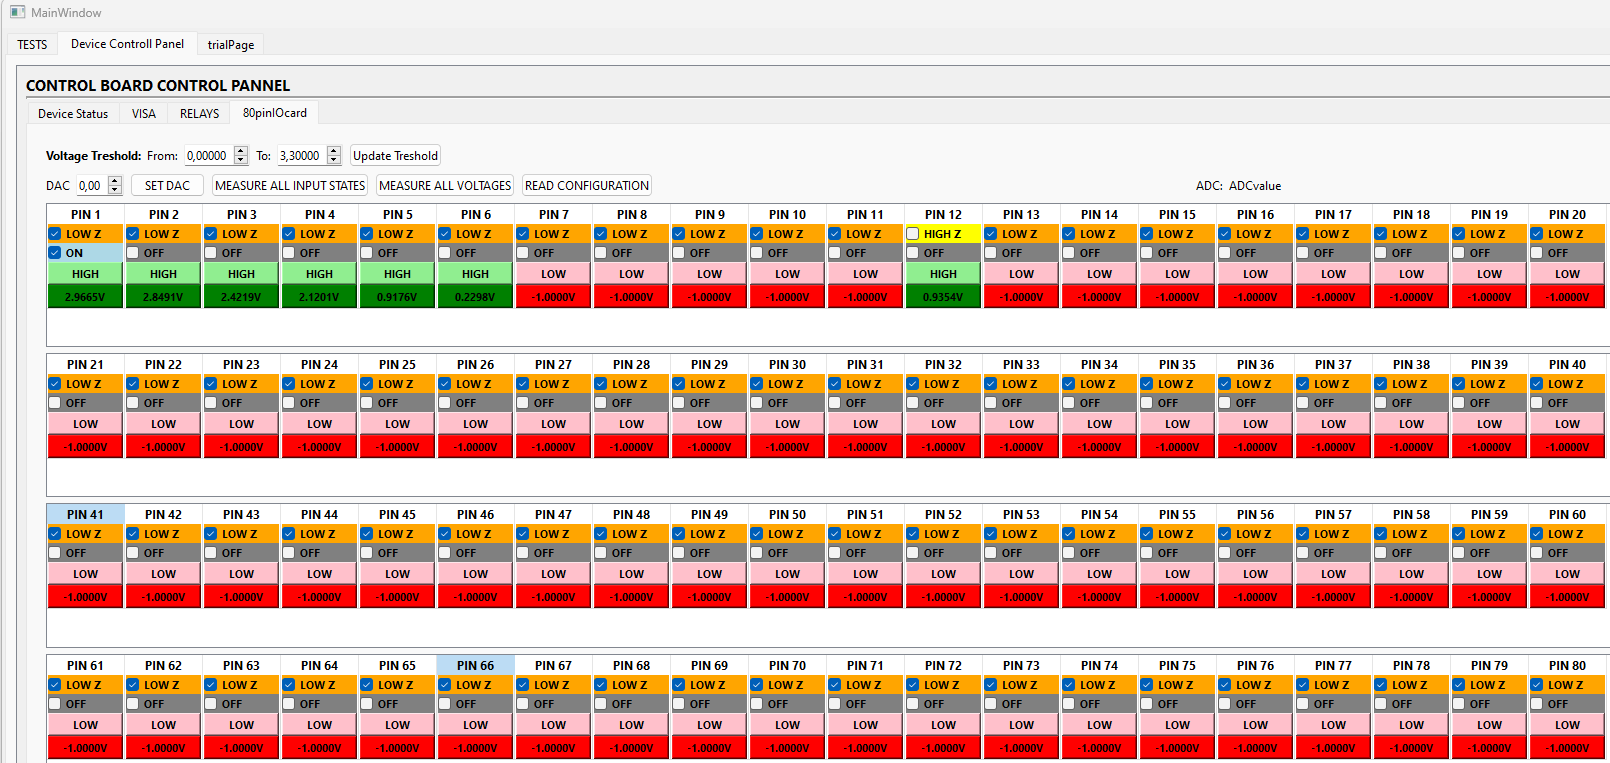
\includegraphics[width = 1\textwidth]{obrazky/PC_APP_CONTROL_PANEL.png}
	\end{figure}
\end{frame}

%%%%%%%%%%%%%
\begin{frame} 
	\frametitle{Pokračování DP}
	\vspace*{0.5cm}
	\begin{itemize}
		\item Finalizace mechanické konstrukce testeru
		\item Ethernet bootloader
		\item Odladění v "ostrém"\ provozu
		\item Ověření dlouhodobé spolehlivosti
		\item Vylepšení CSS stylů PC aplikace
		\item Rozšíření PC aplikace
	\end{itemize}
\end{frame}


% podekovani
\begin{frame}[c] 
% bez nadpisu snímku
	\frametitle{\mbox{ }}
	\begin{center}
		{\Huge Děkuji za pozornost!}
	\end{center}
\end{frame}


% otázky oponenta
\frame{
\frametitle{Otázky oponenta}
\begin{itemize}
	\item \textbf{Uveďte, na kterých částech zařízení jste pracoval sám a zda jste u některých bloků využil spolupráci s kolegy z firmy.}\\
	\item \textbf{Jak často se bude provádět kalibrace zařízení, jednou po sestavení převodníku nebo periodicky?}\\
	\item \textbf{Proč nebyla pro měření použita metoda postupné aproximace (půlení intervalu)? Bylo by takto možné urychlit měření přesného odporu?}\\
\end{itemize}
}

\frame{
\frametitle{Otázky oponenta - Spolupráce kolegů}
\vspace*{1.5cm}
\begin{center}
	{\Huge Uveďte, na kterých částech zařízení jste pracoval sám a zda jste u některých bloků využil spolupráci s kolegy z firmy.}
\end{center}
}

\begin{frame} 
	% nadpis snímku
	\frametitle{Spolupráce kolegů}
	\begin{figure}[ht!]
		\centering
		%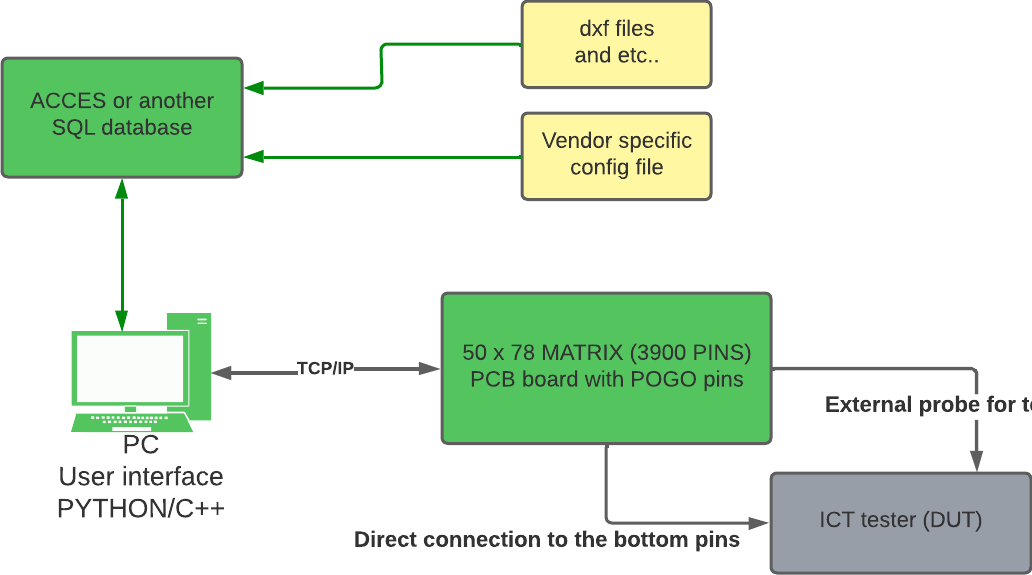
\includegraphics[width = \textwidth]{obrazky/system_connection.png}
		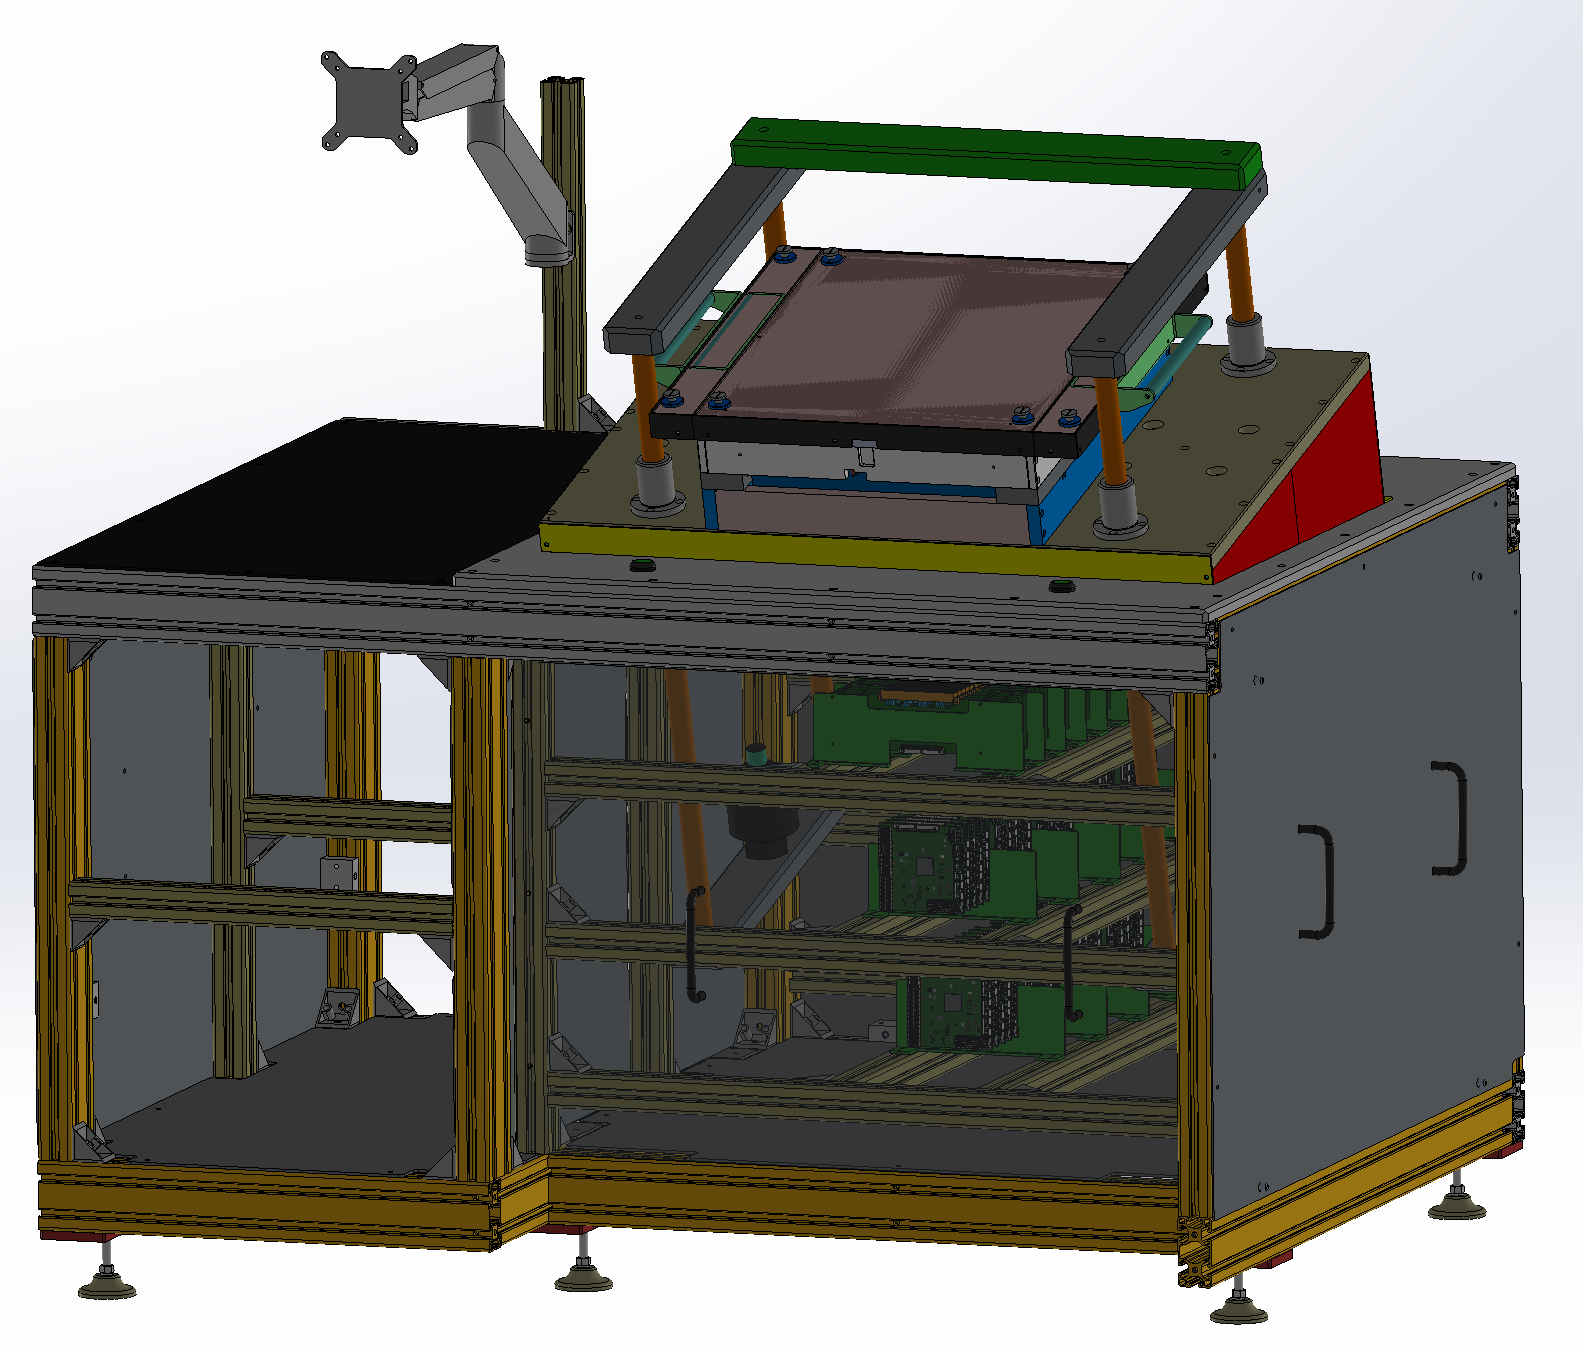
\includegraphics[height = 0.8\textheight]{obrazky/assembly_3D_model.png}
	\end{figure}
\end{frame}


\frame{
\frametitle{Otázky oponenta - Kalibrace}
\vspace*{1.5cm}
\begin{center}
	{\Huge Jak často se bude provádět kalibrace zařízení, jednou po sestavení převodníku nebo periodicky?}
\end{center}
}

\begin{frame} 
	% nadpis snímku
	\frametitle{Otázky oponenta - Kalibrace}
	\vspace*{1.2cm}
	\begin{figure}[ht!]
		\centering
		%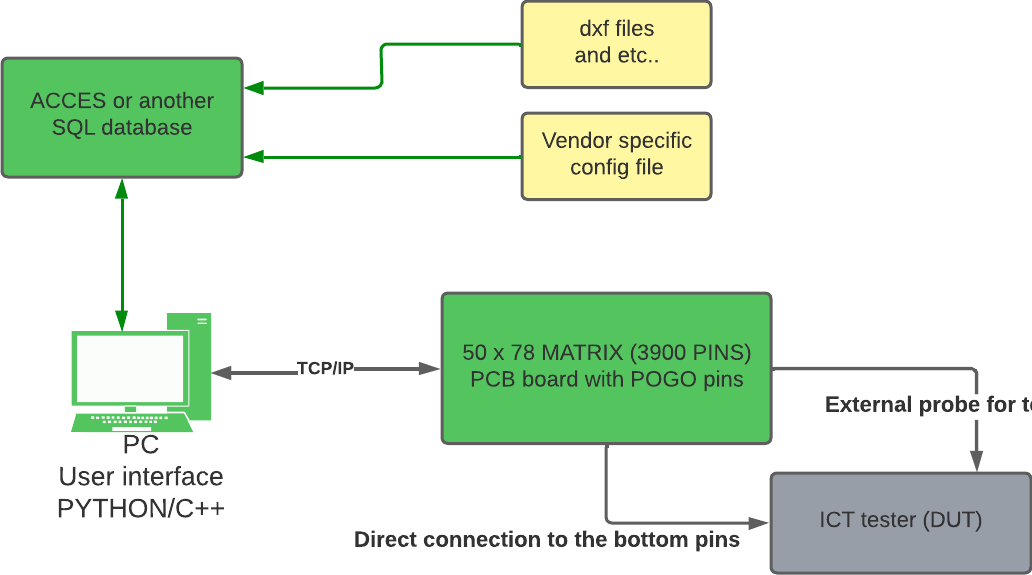
\includegraphics[width = \textwidth]{obrazky/system_connection.png}
		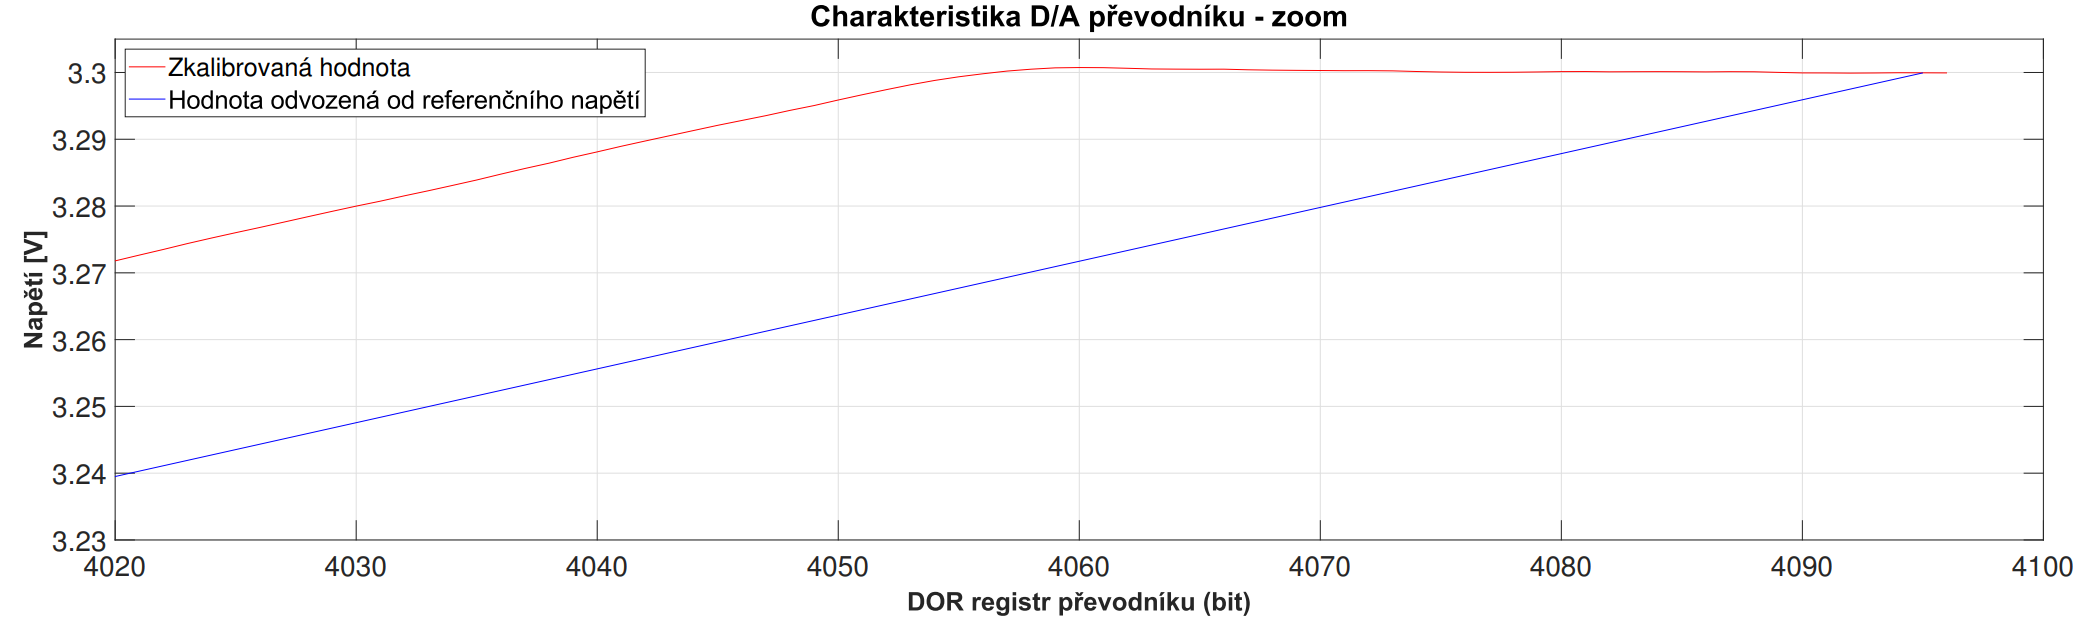
\includegraphics[width = \textwidth]{obrazky/kalibrace_obh.png}
	\end{figure}
\end{frame}

\frame{
\frametitle{Otázky oponenta - metoda postupné aproximace}
\vspace*{1.5cm}
\begin{center}
	{\Huge Proč nebyla pro měření použita metoda postupné aproximace (půlení intervalu)? Bylo by takto možné urychlit měření přesného odporu?}
\end{center}
}

\begin{frame} 
	% nadpis snímku
	\frametitle{Otázky oponenta - metoda postupné aproximace 1/4}
	\vspace*{0.5cm}
	\begin{figure}[ht!]
		\centering
		%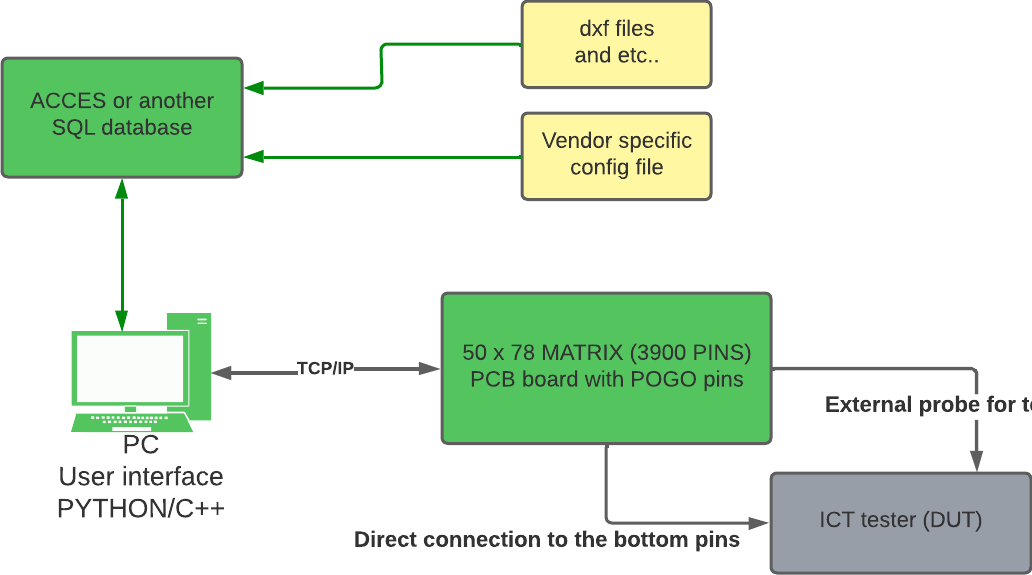
\includegraphics[width = \textwidth]{obrazky/system_connection.png}
		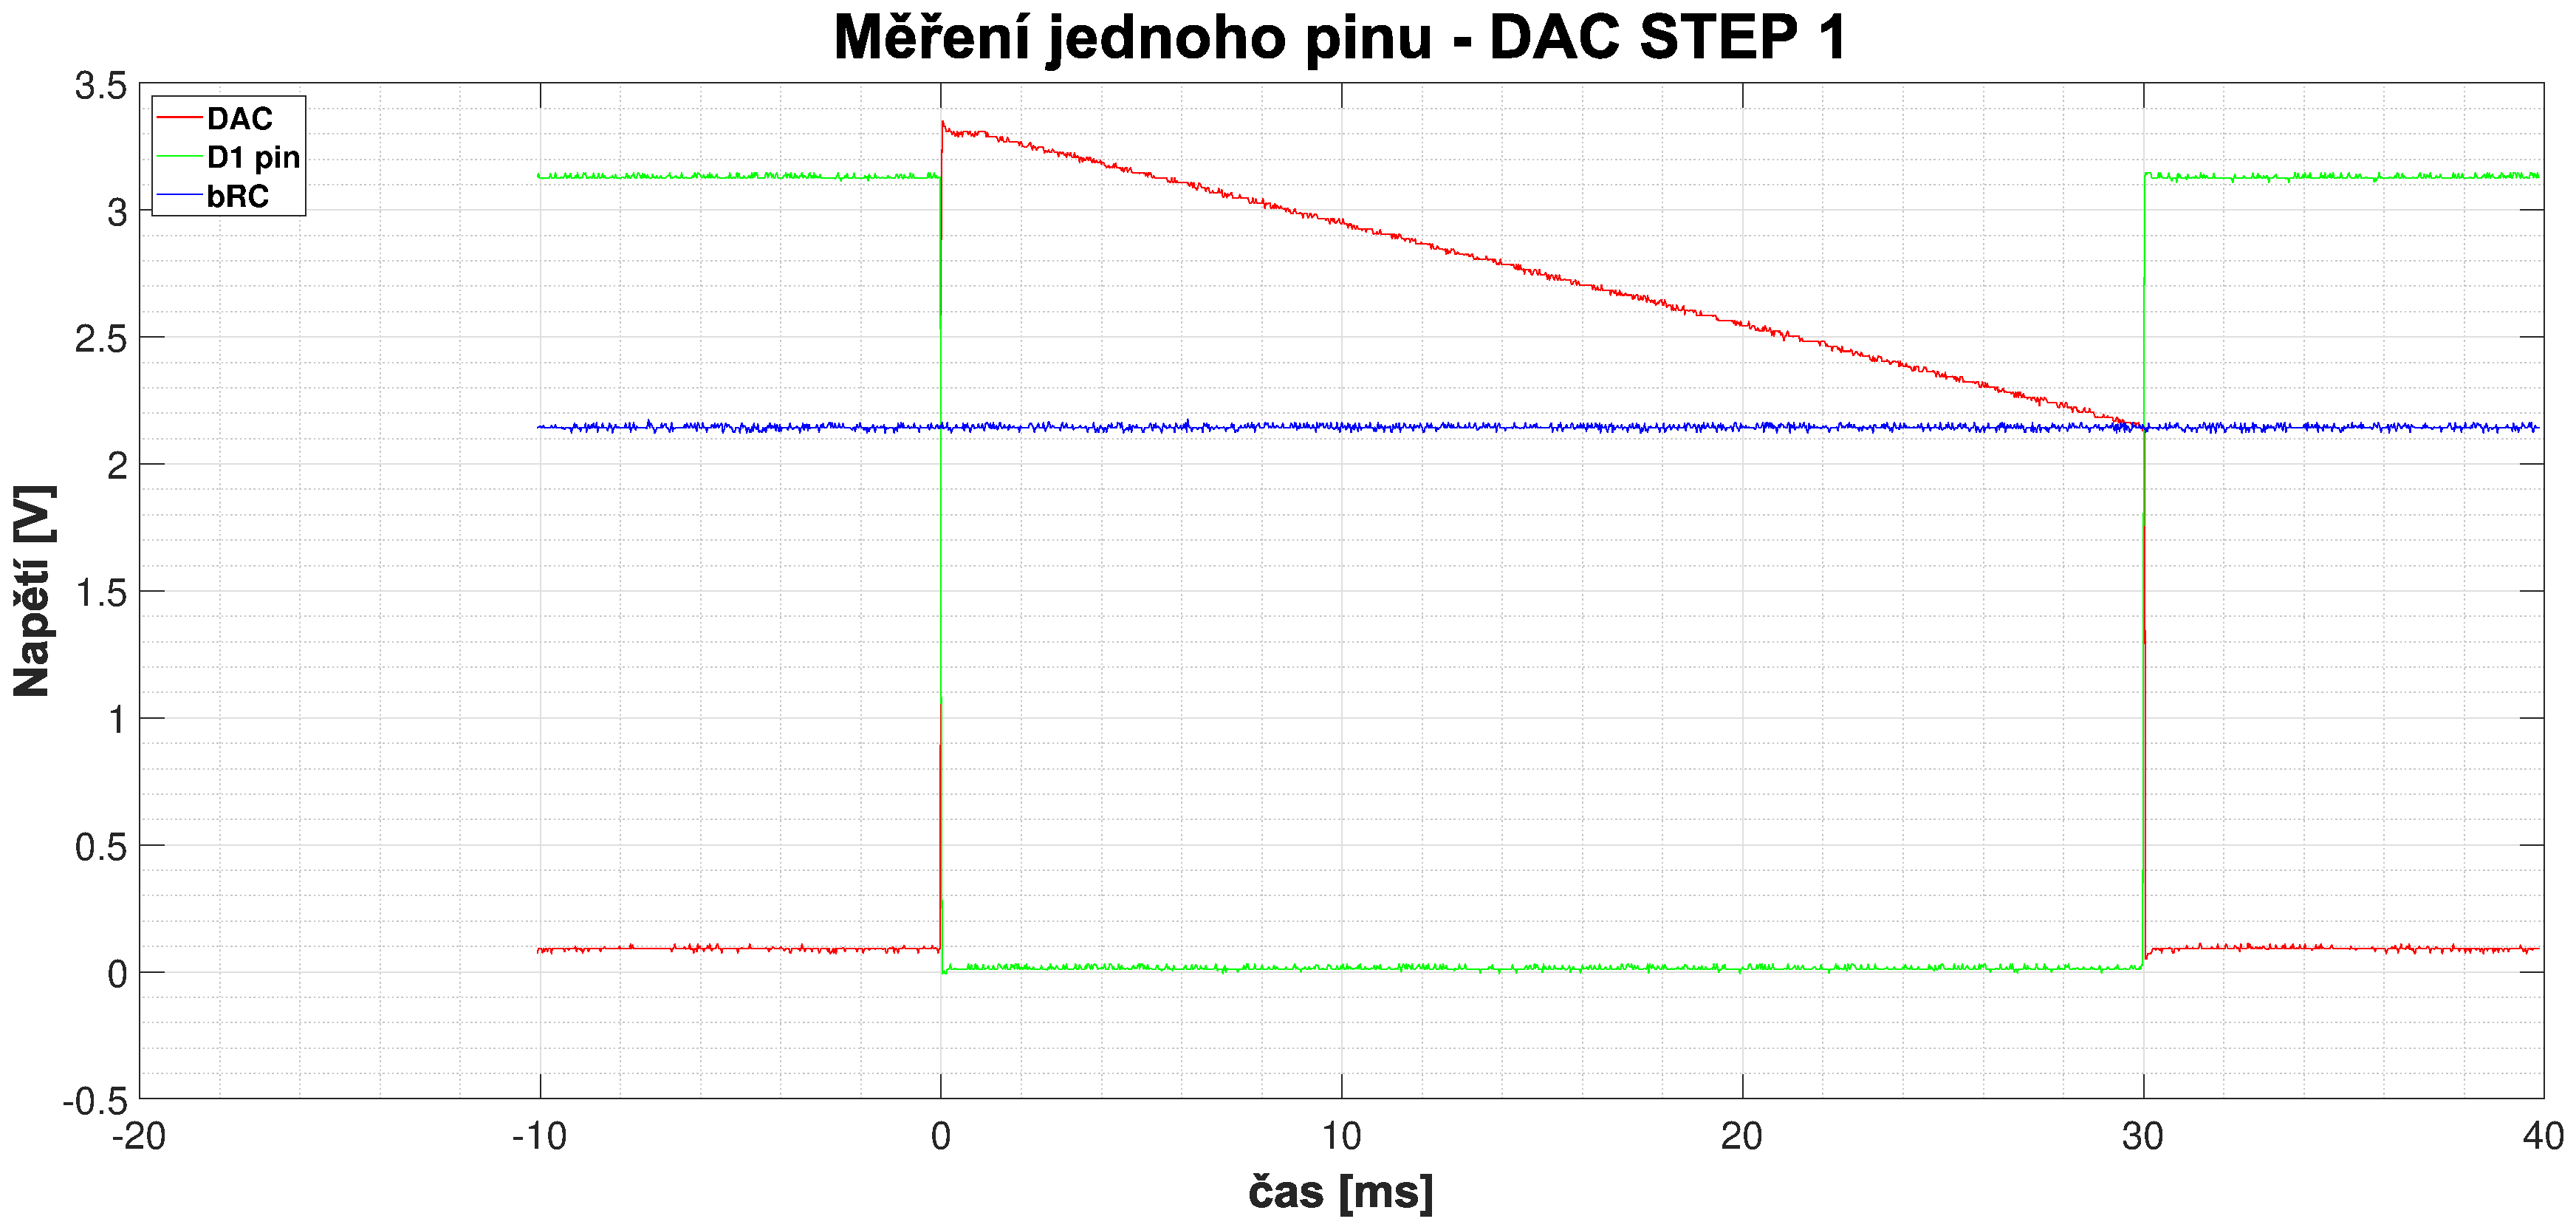
\includegraphics[width = \textwidth]{obrazky/matlab_generated/pin_step1.eps}
	\end{figure}
\end{frame}

\begin{frame} 
	% nadpis snímku
	\frametitle{Otázky oponenta - metoda postupné aproximace 2/4}
	\vspace*{0.5cm}
	\begin{figure}[ht!]
		\centering
		%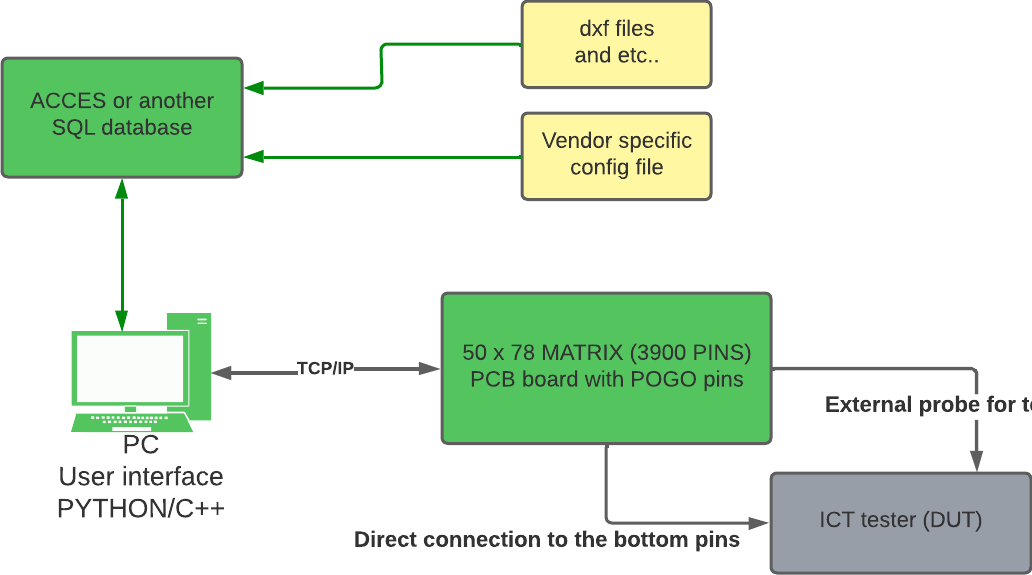
\includegraphics[width = \textwidth]{obrazky/system_connection.png}
		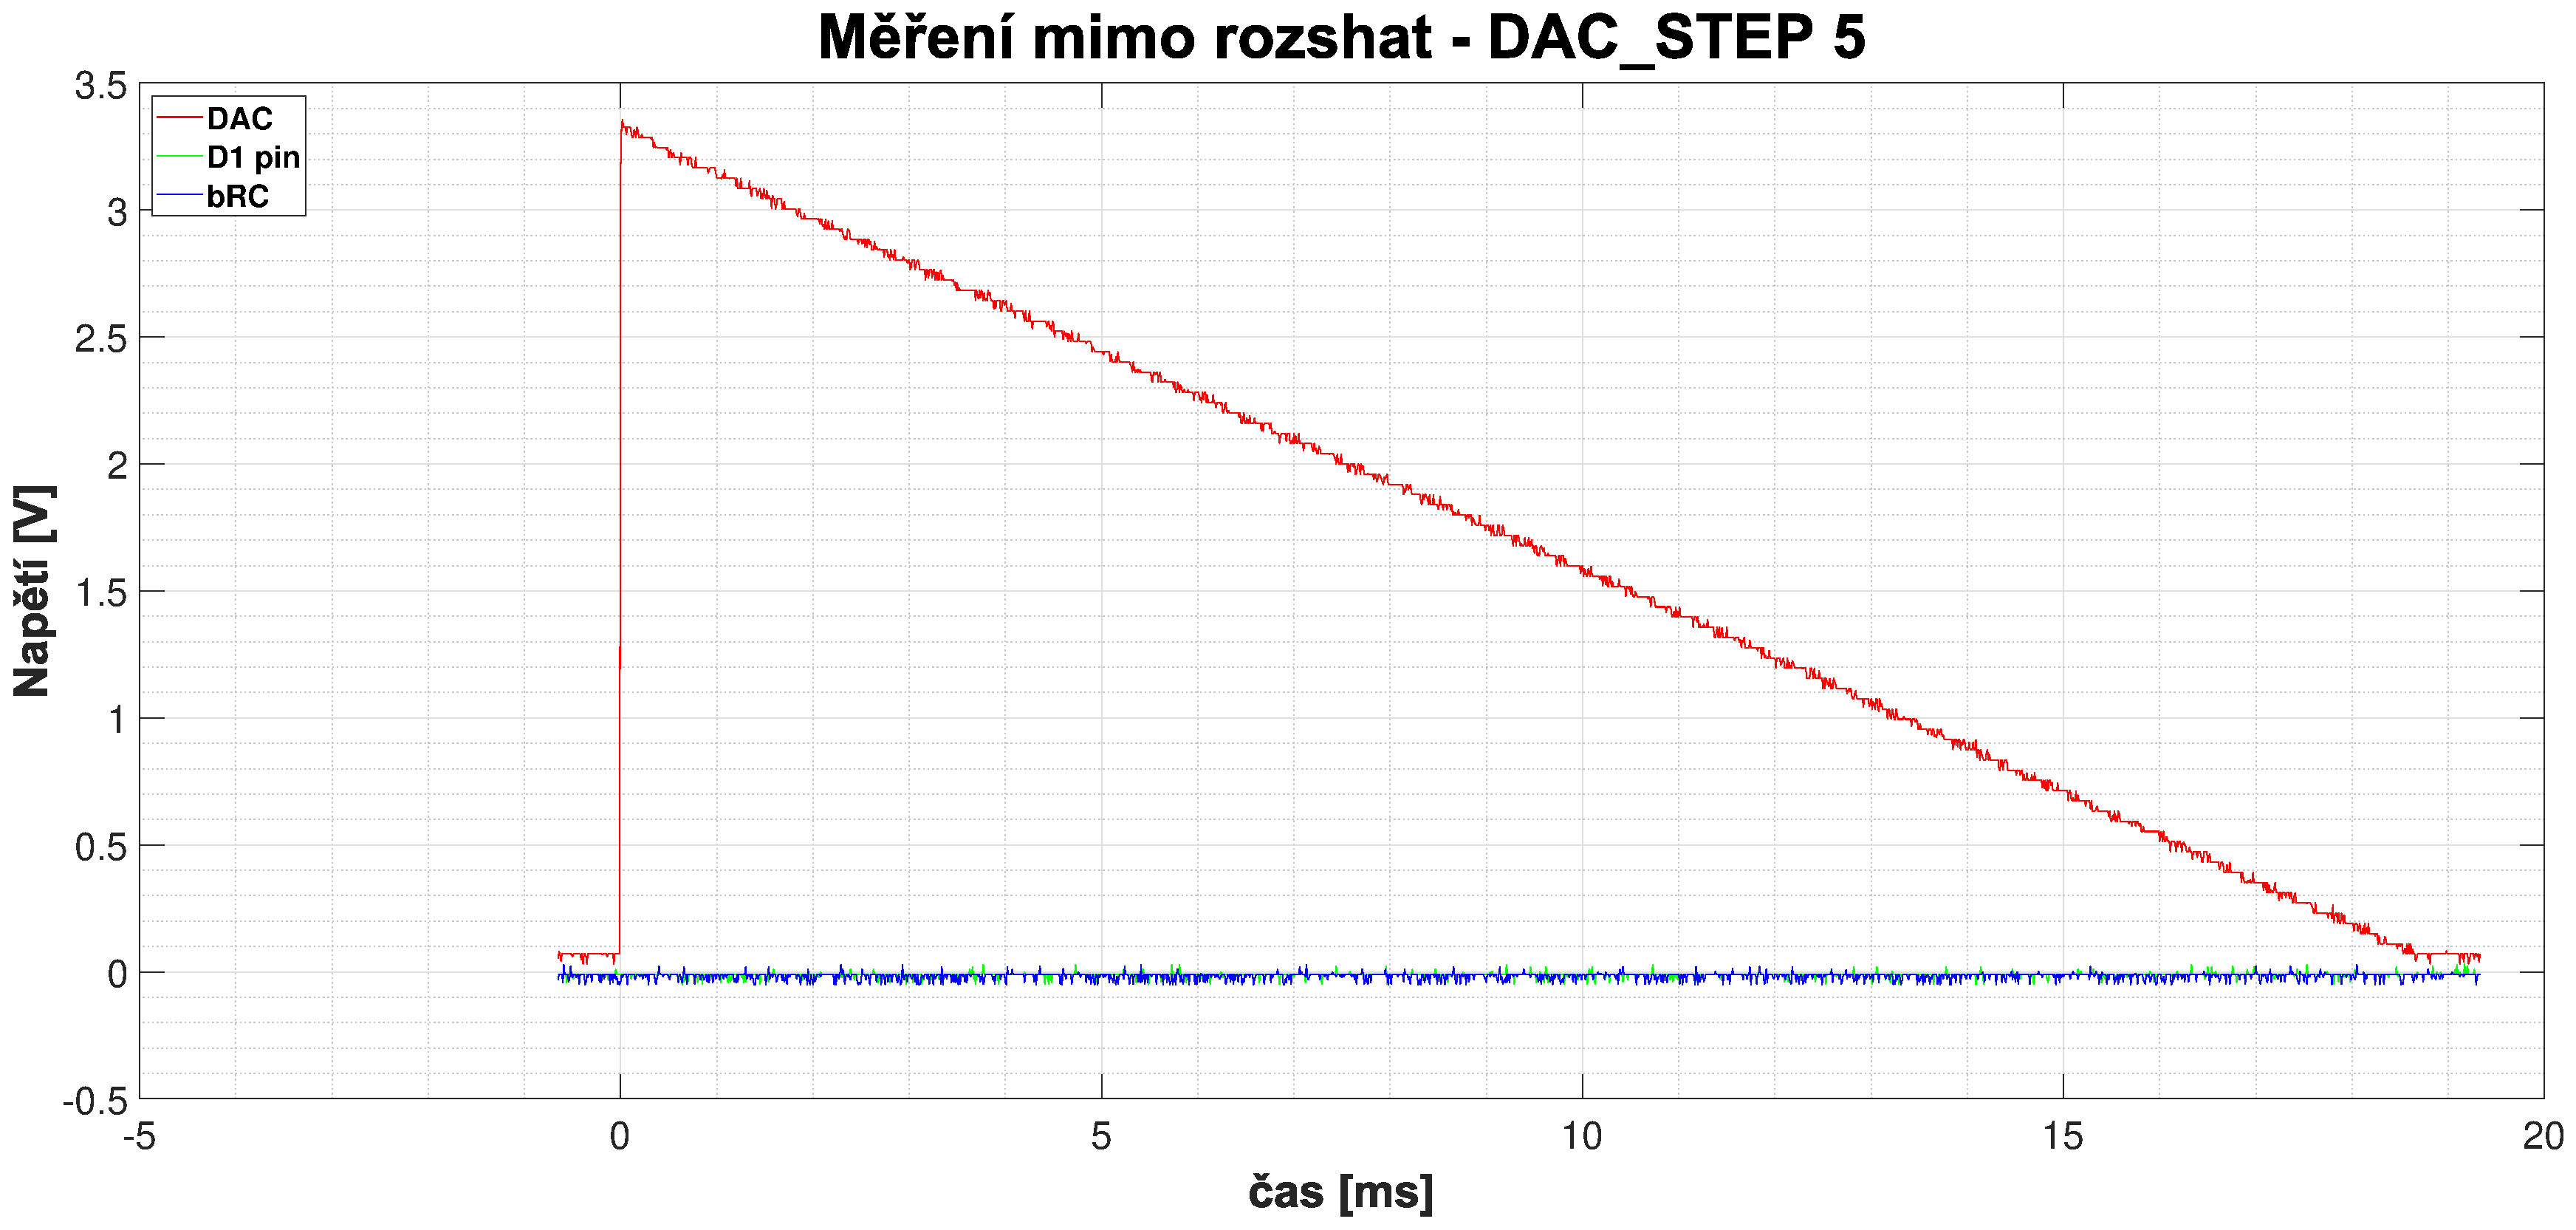
\includegraphics[width = \textwidth]{obrazky/matlab_generated/pin_out_of_range.eps}
	\end{figure}
\end{frame}


\begin{frame} 
	% nadpis snímku
	\frametitle{Otázky oponenta - metoda postupné aproximace 3/4}
	\vspace*{0.5cm}
	\begin{figure}[ht!]
		\centering
		%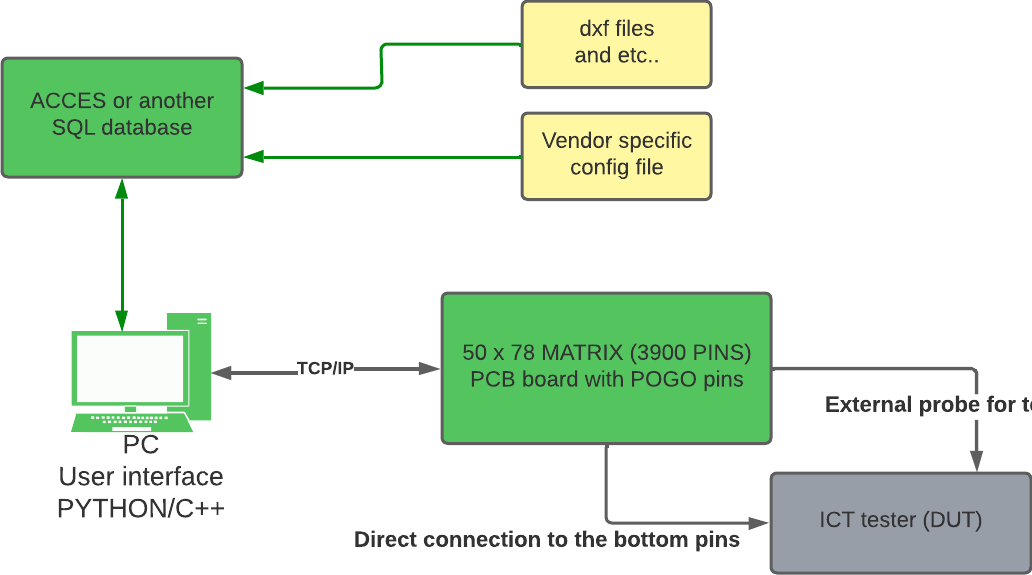
\includegraphics[width = \textwidth]{obrazky/system_connection.png}
		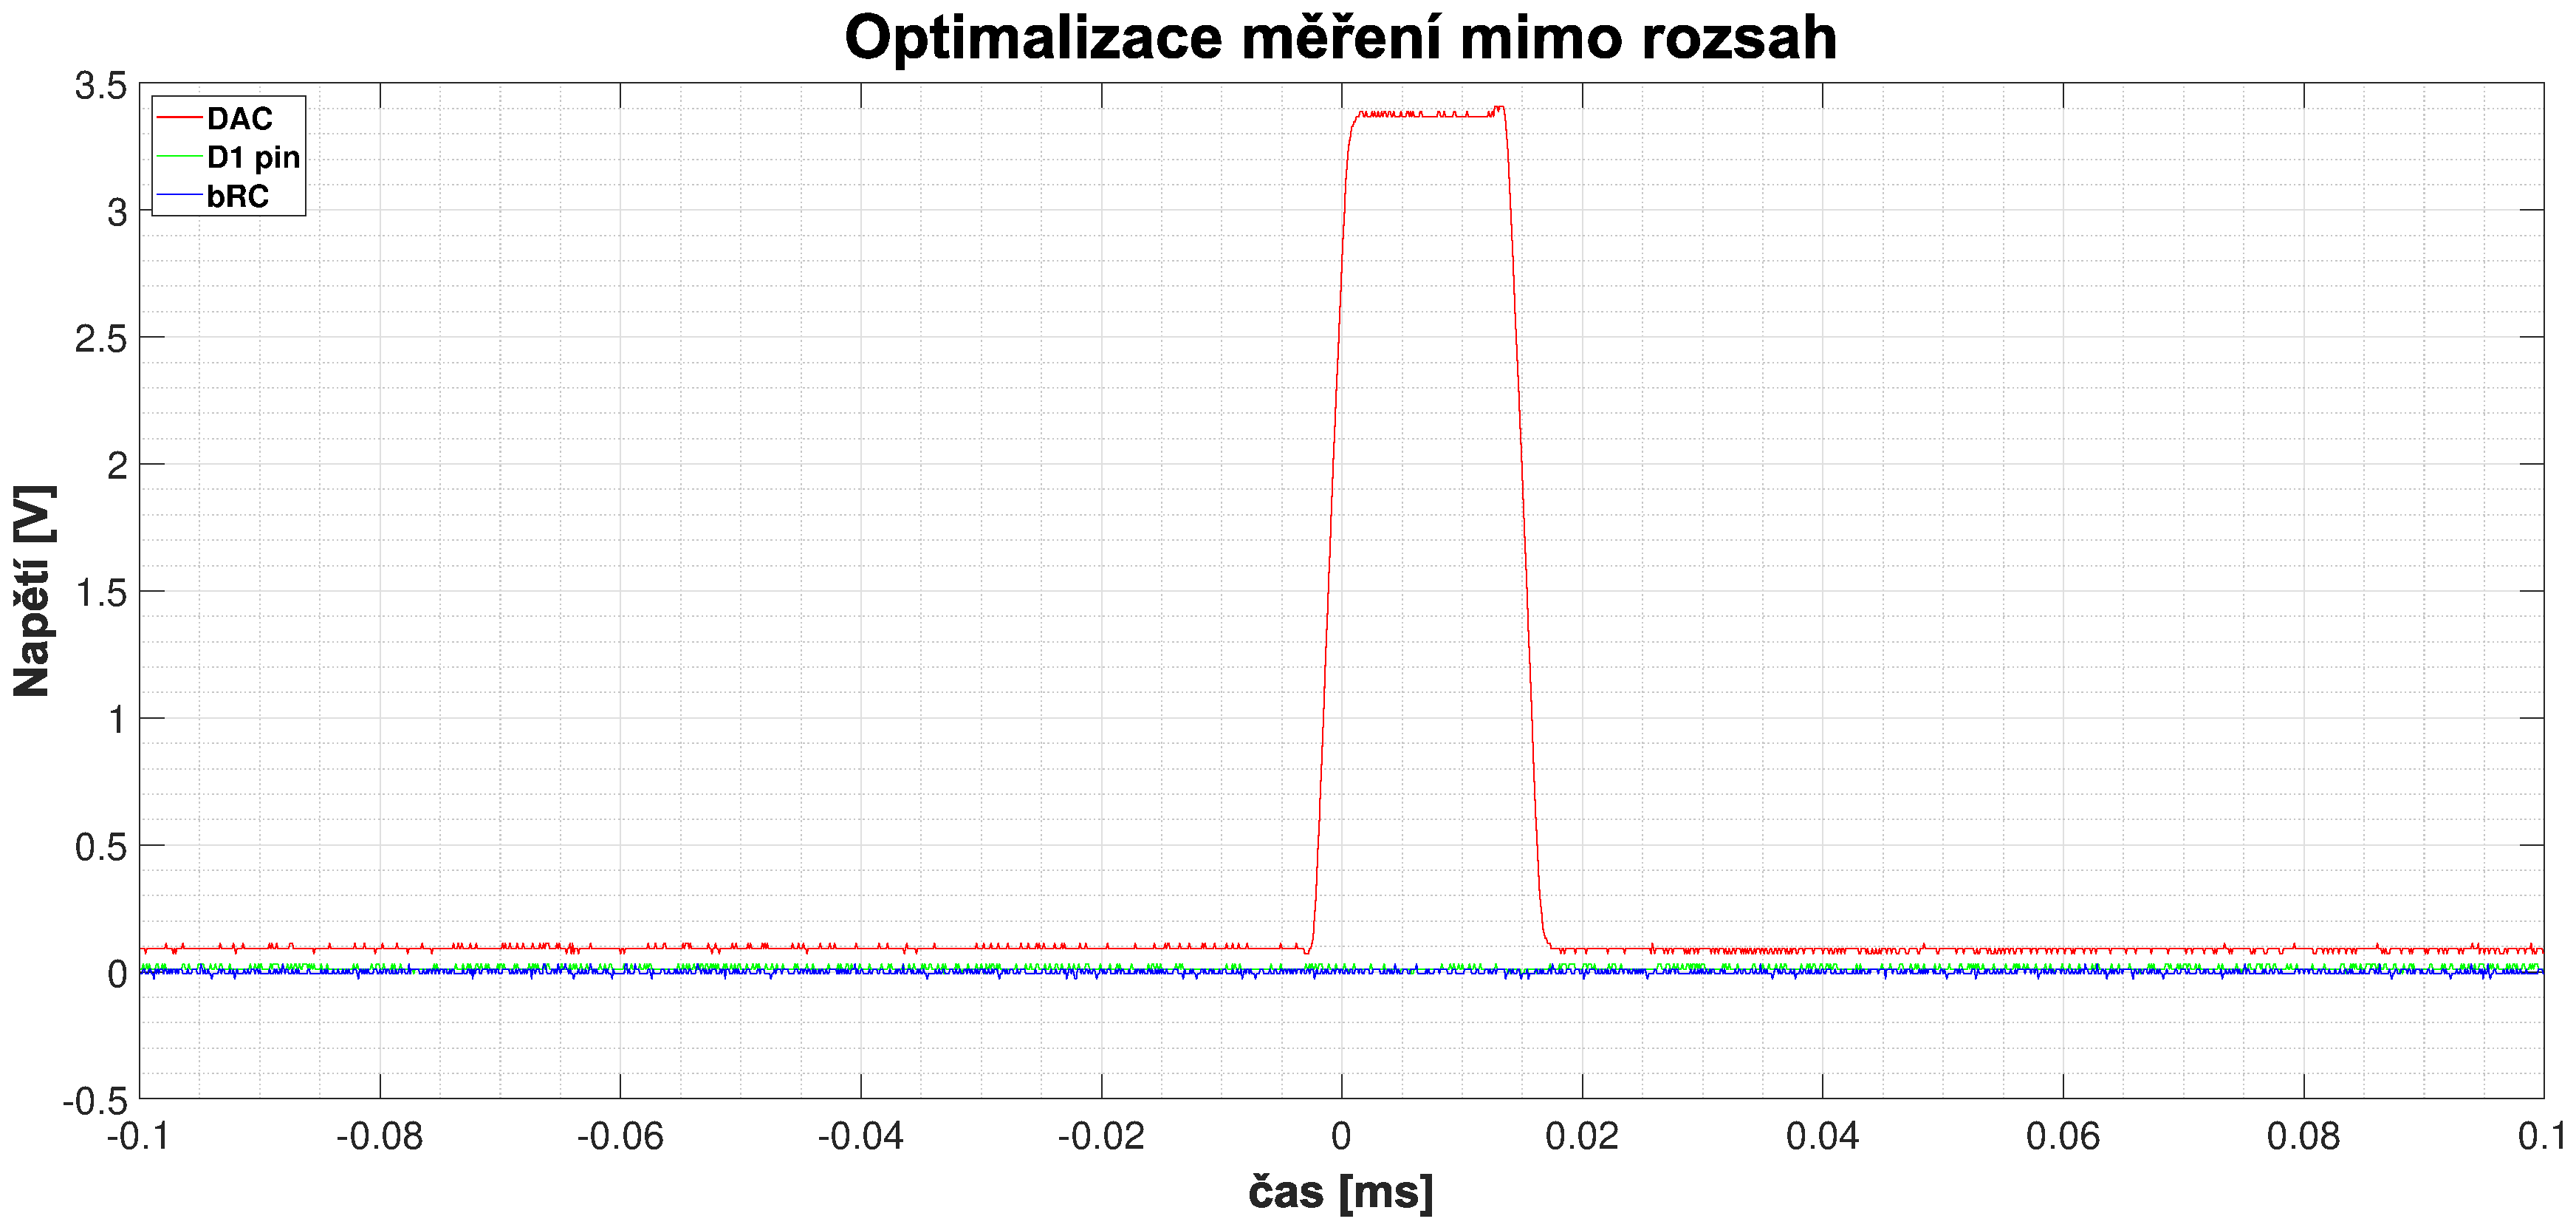
\includegraphics[width = \textwidth]{obrazky/matlab_generated/pin_out_of_range_opt.eps}
	\end{figure}
\end{frame}


\begin{frame} 
	% nadpis snímku
	\frametitle{Otázky oponenta - metoda postupné aproximace 4/4}
	\vspace*{0.5cm}
	\begin{figure}[ht!]
		\centering
		%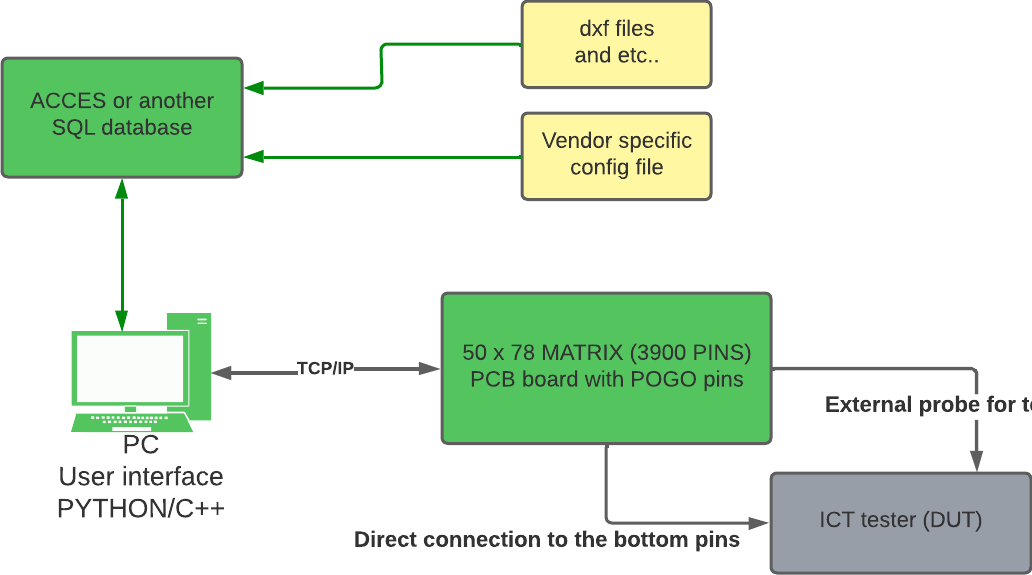
\includegraphics[width = \textwidth]{obrazky/system_connection.png}
		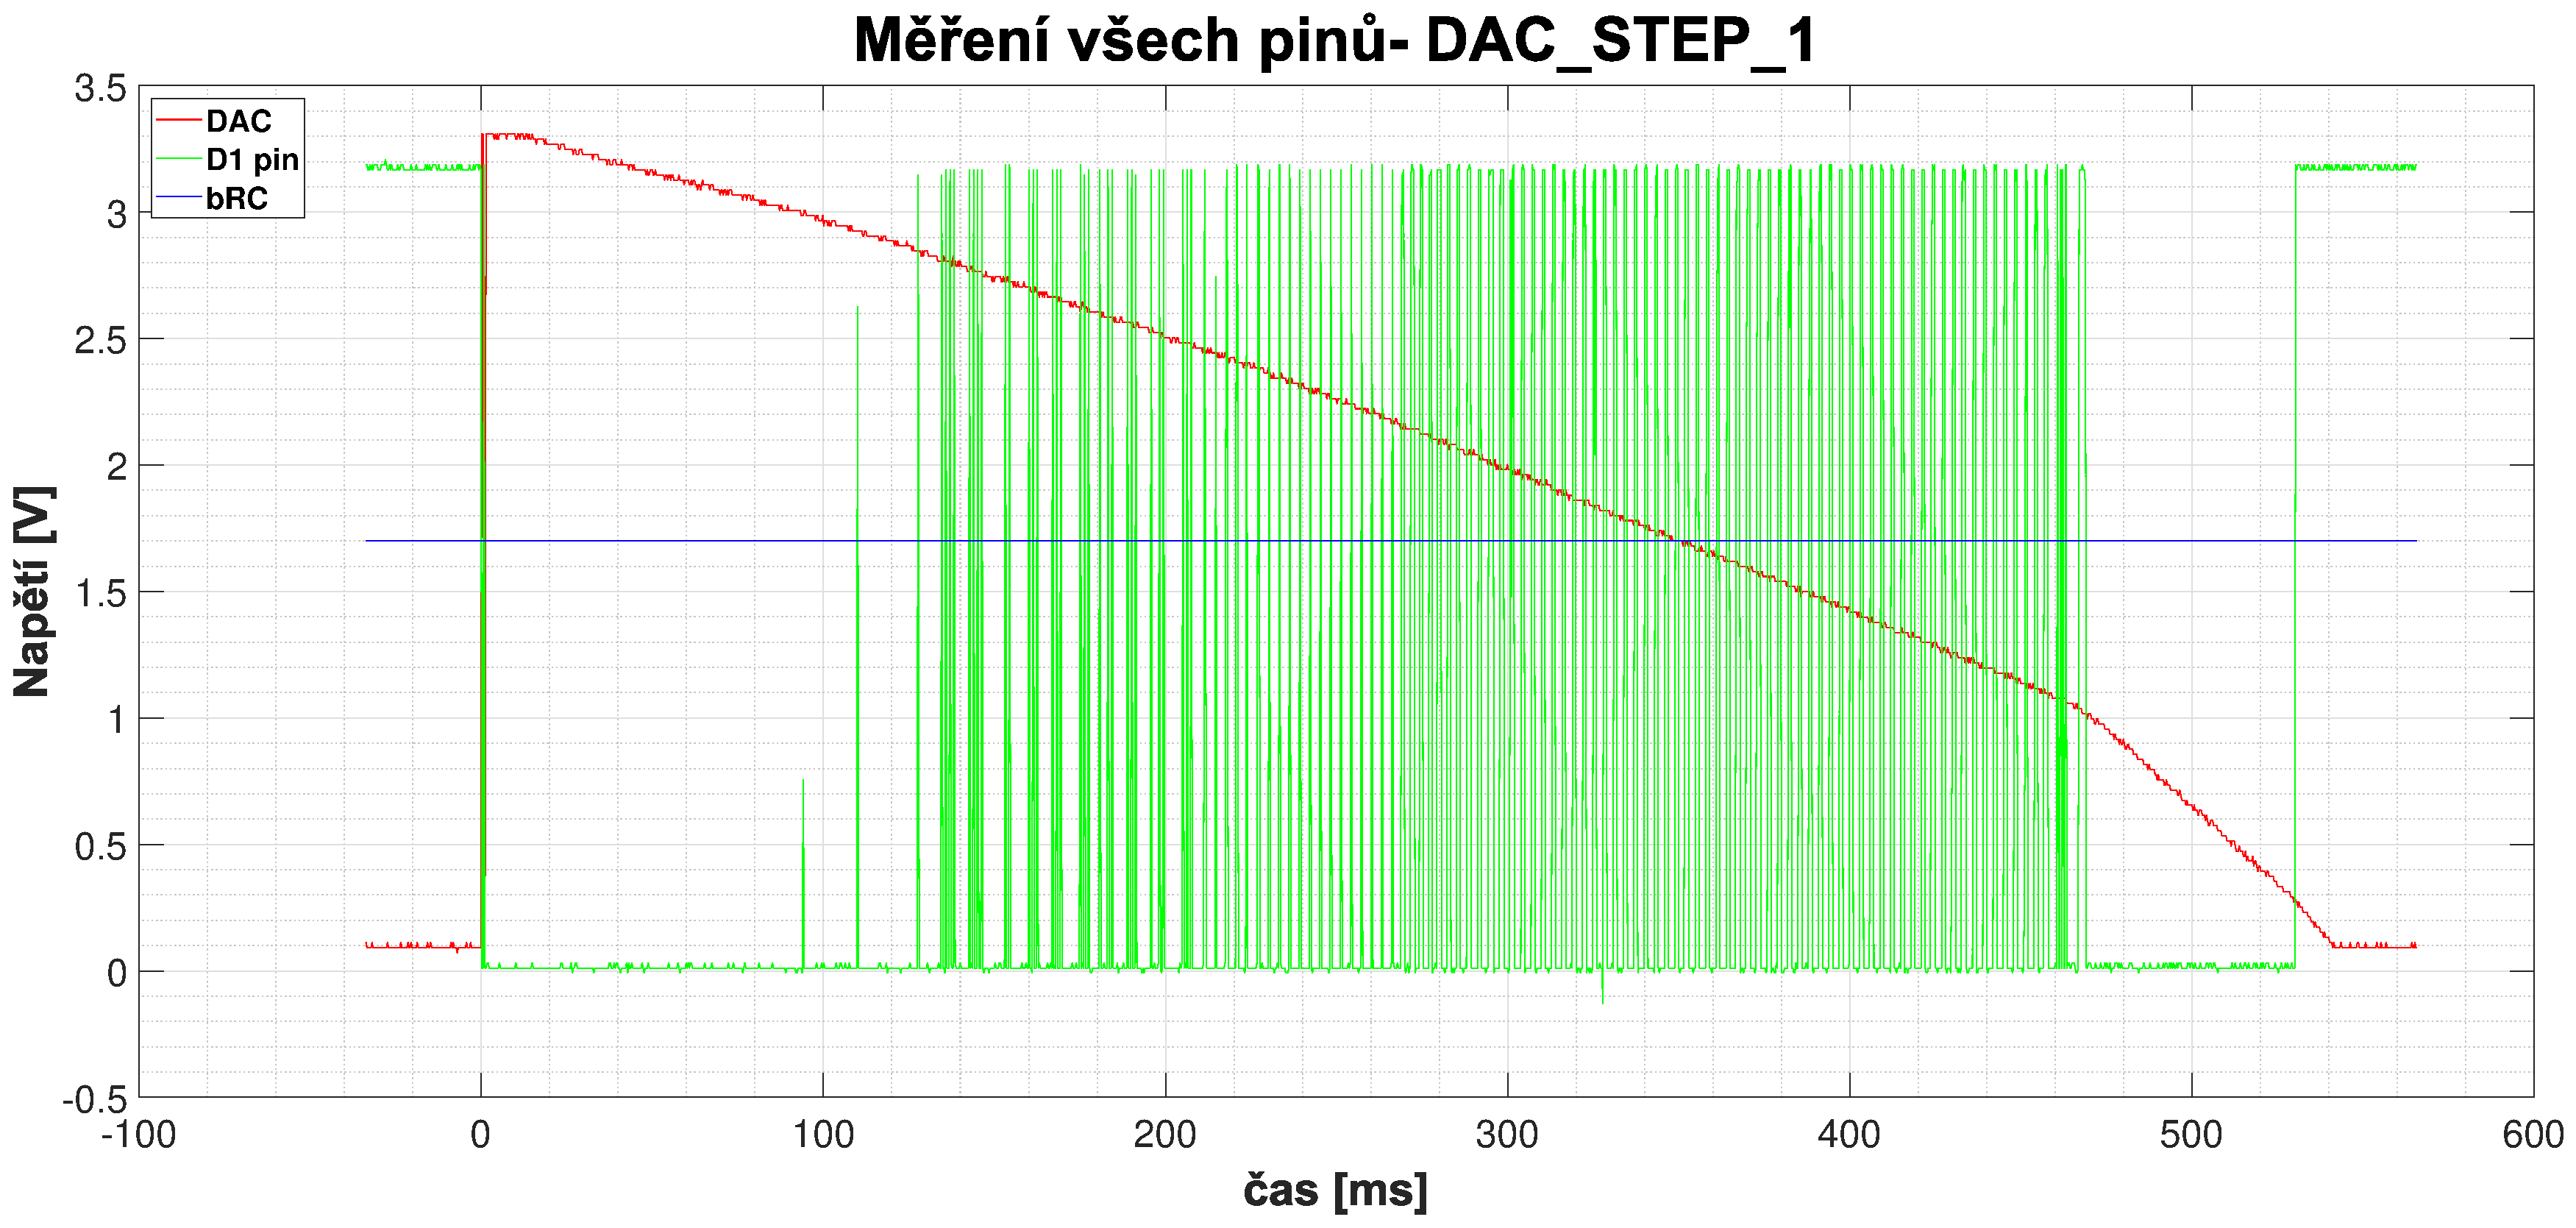
\includegraphics[width = \textwidth]{obrazky/matlab_generated/all_pins.eps}
	\end{figure}
\end{frame}


\end{document}
